\documentclass[conference]{IEEEtran}
\IEEEoverridecommandlockouts

\usepackage{cite}
\usepackage{amsmath,amssymb,amsfonts}
\usepackage{algorithmic}
\usepackage{graphicx}
\usepackage{textcomp}
\usepackage{xcolor}
\usepackage{booktabs}
\usepackage{multirow}
\usepackage{hyperref}

\def\BibTeX{{\rm B\kern-.05em{\sc i\kern-.025em b}\kern-.08em
    T\kern-.1667em\lower.7ex\hbox{E}\kern-.125emX}}

\begin{document}

\title{Analysis of Cigarette and Marijuana Use Patterns: A Comprehensive Statistical Investigation Using the National Survey on Drug Use and Health 2012}

\author{\IEEEauthorblockN{Hasan Alper AYAZ}
\IEEEauthorblockA{\textit{Computer Engineering} \\
\textit{Galatasaray University}\\
Istanbul, Turkey}
}

\maketitle

\begin{abstract}
This study presents a comprehensive analysis of cigarette and marijuana use patterns among the U.S. civilian population using data from the National Survey on Drug Use and Health (NSDUH) 2012. The dataset comprises 55,268 respondents aged 12 and older, providing detailed information on substance use behaviors, risk perceptions, dependence indicators, and mental health outcomes. Our analysis reveals that 50.4\% of respondents have ever smoked cigarettes, while 40.2\% have used marijuana at least once. Significant demographic variations exist, with prevalence increasing dramatically from adolescence (18.6\% for cigarettes, 17.8\% for marijuana among 12-17 year-olds) to young adulthood (60.7\% and 52.6\% among 18-25 year-olds). Males initiate use significantly earlier than females for both substances (p $<$ 0.001). Strong inverse correlations exist between risk perception and use behaviors (r = -0.461 for marijuana). Cigarette smoking frequency strongly predicts dependence symptoms (r = 0.587, p $<$ 0.001), with daily smokers showing mean dependence scores more than twice those of occasional smokers. Substance use is significantly associated with mental distress (F = 263.26, p $<$ 0.001), with dual users exhibiting the highest distress levels. Remarkably, the odds of marijuana use are 14.20 times higher among cigarette users (OR = 14.20), with 34\% of the sample reporting use of both substances. These findings underscore the importance of early intervention, integrated prevention strategies, and addressing mental health in substance abuse treatment.
\end{abstract}

\begin{IEEEkeywords}
substance abuse, cigarette smoking, marijuana use, drug prevention, risk perception, mental health, NSDUH, statistical analysis, predictive modeling
\end{IEEEkeywords}

\section{Introduction}

\subsection{Overview}

Substance abuse remains a critical public health challenge in the United States, contributing to significant morbidity, mortality, and economic burden. Cigarette smoking and marijuana use represent two of the most prevalent forms of substance use, each associated with distinct health risks and societal impacts. Understanding the patterns, predictors, and correlates of these behaviors is essential for developing effective prevention and intervention strategies.

Cigarette smoking continues to be the leading preventable cause of death in the United States, responsible for more than 480,000 deaths annually \cite{cdc2014}. Despite decades of public health efforts, including smoking cessation programs, taxation policies, and anti-smoking campaigns, smoking prevalence remains substantial, particularly among certain demographic groups. Marijuana use has also increased in recent years, particularly following changes in legal status across various states, making it crucial to understand contemporary use patterns and their implications.

The National Survey on Drug Use and Health (NSDUH) provides one of the most comprehensive data sources for understanding substance use behaviors in the United States. Conducted annually by the Substance Abuse and Mental Health Services Administration (SAMHSA), the NSDUH employs a multistage area probability sampling design to obtain nationally representative estimates of substance use, abuse, and dependence among the civilian, noninstitutionalized population aged 12 and older.

\subsection{Motivation}

Several factors motivate this analysis of cigarette and marijuana use patterns. First, the co-occurrence of cigarette and marijuana use is common, yet the interrelationships between these behaviors remain incompletely understood. Understanding how use of one substance relates to use of another can inform integrated prevention and treatment approaches.

Second, the age of initiation for substance use is a critical predictor of later problematic use and dependence. Early initiation is associated with increased risk of developing substance use disorders, experiencing negative health outcomes, and engaging in other risky behaviors. By examining the distribution of initiation ages and their correlates, we can identify high-risk periods for targeted intervention.

Third, risk perception plays a crucial role in substance use decisions. Individuals who perceive greater risk associated with substance use are generally less likely to engage in such behaviors. However, risk perceptions can be influenced by various factors, including personal experience, social norms, and public health messaging. Understanding the relationship between risk perception and actual use behaviors can inform communication strategies.

Fourth, the relationship between substance use and mental health is bidirectional and complex. Individuals may use substances to self-medicate mental health symptoms, while substance use itself can exacerbate or precipitate mental health problems. Examining these relationships at the population level can provide insights into the mental health burden associated with substance use.

Finally, demographic factors such as age, gender, and socioeconomic status are known to be associated with substance use patterns. Understanding these demographic variations is essential for targeting prevention efforts to the populations at greatest risk.

\subsection{Research Questions}

This study addresses the following research questions:

\begin{enumerate}
    \item \textbf{RQ1: Prevalence and Patterns}: What is the prevalence of cigarette and marijuana use in the U.S. population, and how do use patterns vary across different demographic groups?
    
    \item \textbf{RQ2: Age of Initiation}: What are the typical ages of initiation for cigarette and marijuana use, and how do these ages vary by demographic characteristics?
    
    \item \textbf{RQ3: Risk Perception}: How do individuals perceive the risks associated with cigarette and marijuana use, and how do these perceptions relate to actual use behaviors?
    
    \item \textbf{RQ4: Dependence and Frequency}: What are the patterns of frequent use and dependence symptoms among cigarette and marijuana users, and what factors are associated with higher levels of dependence?
    
    \item \textbf{RQ5: Mental Health Correlates}: What is the relationship between substance use and mental health indicators such as nervousness, hopelessness, and restlessness?
    
    \item \textbf{RQ6: Co-occurrence}: To what extent do cigarette and marijuana use co-occur, and what factors are associated with polysubstance use?
\end{enumerate}

\subsection{Contributions}

This study makes several key contributions to the literature on substance use epidemiology. First, we describe prevalence and patterns of cigarette and marijuana use in a large national survey sample. Second, we conduct comprehensive statistical analyses examining demographic, behavioral, and psychological correlates of substance use. Third, we quantify the relationship between risk perception and use behaviors, providing insights for prevention messaging. Fourth, we characterize dependence patterns among cigarette smokers and their relationship to use frequency. Fifth, we examine the mental health burden associated with substance use, including polysubstance use. Finally, we document the strong co-occurrence between cigarette and marijuana use, highlighting the need for integrated prevention and treatment approaches.

\section{Method}

\subsection{Dataset}

\subsubsection{Story and Overview}

The National Survey on Drug Use and Health (NSDUH) 2012 is a comprehensive, nationally representative survey that measures the prevalence and correlates of drug use in the United States. Originally titled the National Household Survey on Drug Abuse, the NSDUH has been conducted annually since 1971, providing crucial data for monitoring trends in substance use and informing policy decisions.

The 2012 survey employed a sophisticated multistage area probability sampling design to ensure representation across all 50 states and the District of Columbia. The survey covers substance use behaviors, treatment history, perceived need for treatment, and includes diagnostic criteria from the Diagnostic and Statistical Manual (DSM) of Mental Disorders. Importantly, the survey also collects information on demographic characteristics, socioeconomic factors, mental health indicators, and behavioral risk factors.

Data collection for the 2012 NSDUH occurred throughout the calendar year, utilizing computer-assisted interviewing methods including audio computer-assisted self-interview (ACASI) for sensitive questions, which has been shown to improve reporting of stigmatized behaviors. Each respondent who completed the survey received a \$30 incentive payment, contributing to a weighted interview response rate of 73.04\%.

The survey universe comprises the civilian, noninstitutionalized population of the United States aged 12 and older. This includes residents of households and noninstitutional group quarters such as college dormitories, group homes, shelters, and rooming houses. The achieved sample size for 2012 was 68,309 persons, with the public use file containing 55,268 records after disclosure protection procedures including data substitution and record subsampling.

\subsubsection{Attributes}

For this analysis, we selected 25 key variables spanning multiple domains relevant to understanding cigarette and marijuana use patterns. Table \ref{tab:variables} provides a comprehensive overview of these variables.

\begin{table*}[t]
\centering
\caption{Selected Variables for Analysis}
\label{tab:variables}
\small
\begin{tabular}{@{}llp{7.5cm}c@{}}
\toprule
\textbf{Category} & \textbf{Variable} & \textbf{Description} & \textbf{Values} \\ \midrule
\multirow{7}{*}{\textbf{Cigarette Use}} 
& CIGEVER & Ever smoked a cigarette & 2 \\
& CIGOFRSM & Would smoke if best friend offered & 7 \\
& CIGTRY & Age when first smoked a cigarette & 55 \\
& CIG30USE & Days smoked cigarettes in past 30 days & 35 \\
& CIG30AV & Average cigarettes per day when smoking & 12 \\
& CIGAGE & Age when first started smoking daily & 60 \\
& CIG100LF & Smoked 100+ cigarettes in lifetime & 7 \\ \midrule

\multirow{4}{*}{\textbf{Marijuana Use}}
& MJEVER & Ever used marijuana/hashish & 5 \\
& MJAGE & Age when first used marijuana & 65 \\
& MJYRTOT & Total days used marijuana in past 12 months & 227 \\
& MRDAYPWK & Days per week used marijuana (past 12 months) & 14 \\ \midrule

\multirow{5}{*}{\textbf{Risk Perception}}
& RSKPKCIG & Perceived risk: smoking 1+ pack/day & 7 \\
& RSKMJREG & Perceived risk: using marijuana 1-2x/week & 7 \\
& RSKDIFMJ & Difficulty obtaining marijuana & 8 \\
& RKFQDNGR & Enjoys doing dangerous things & 7 \\
& RKFQPBLT & Frequency of wearing seatbelt & 7 \\ \midrule

\multirow{2}{*}{\textbf{Dependence}}
& CIGIRTBL & Need cigarettes to feel less irritable & 10 \\
& CIGCRAVE & Crave cigarettes after few hours & 10 \\ \midrule

\textbf{Acquisition} & MMGETMJ & How obtained last marijuana used & 10 \\ \midrule

\multirow{3}{*}{\textbf{Mental Health}}
& DSTNRV30 & Felt nervous in past 30 days & 9 \\
& DSTHOP30 & Felt hopeless in past 30 days & 9 \\
& DSTRST30 & Felt restless/fidgety in past 30 days & 9 \\ \midrule

\multirow{3}{*}{\textbf{Demographics}}
& CATAGE & Age category (4 groups) & 4 \\
& SEXAGE & Gender by age category & 5 \\
& WRKBZCA2 & Employment business category & 12 \\ \bottomrule
\end{tabular}
\end{table*}

The cigarette use variables capture lifetime use (CIGEVER), experimental use (CIGTRY), transition to regular use (CIGAGE, CIG100LF), and recent use patterns (CIG30USE, CIG30AV). The willingness to smoke if offered by a friend (CIGOFRSM) provides insight into susceptibility to social influences.

Marijuana use variables parallel the cigarette variables, including lifetime use (MJEVER), age of initiation (MJAGE), and frequency of use over different time periods (MJYRTOT, MRDAYPWK). The acquisition variable (MMGETMJ) provides information about how users obtain marijuana, which has implications for understanding social networks and potential intervention points.

Risk perception variables assess individuals' beliefs about the harmfulness of regular cigarette and marijuana use, as well as the perceived difficulty of obtaining marijuana. General risk-taking propensity is captured through questions about enjoying dangerous activities and seatbelt use.

Dependence indicators focus on cigarette smoking, measuring two key symptoms of nicotine dependence: using cigarettes to regulate mood (CIGIRTBL) and experiencing cravings (CIGCRAVE). These symptoms are important predictors of difficulty quitting.

Mental health variables assess the frequency of experiencing common psychological distress symptoms in the past 30 days, including nervousness, hopelessness, and restlessness. These measures allow examination of associations between substance use and mental health.

Demographic variables enable stratified analyses by age group, gender, and employment sector, allowing us to identify populations at higher risk for substance use.

\subsection{Methods for Answering Research Questions}

To address our research questions, we employed a comprehensive analytical strategy combining descriptive statistics, inferential statistics, and visualization techniques.

\subsubsection{Data Preparation}

Prior to analysis, we performed several data preprocessing steps. Binary indicators were created for lifetime use of cigarettes (CIGEVER = 1) and marijuana (MJEVER = 1). Age of initiation variables were cleaned by recoding missing value indicators (values $\geq$ 100) to missing. A composite mental distress score was created by summing the reverse-coded frequencies of nervousness, hopelessness, and restlessness (range: 3-15, higher scores indicate greater distress). For cigarette smokers, a dependence score was calculated by summing irritability and craving frequency scores (range: 2-10, higher scores indicate greater dependence). NSDUH special codes (e.g., 85, 91, 93, 94, 97, 98, 99 for skips, don't know, refused, or blank) were treated as missing. Note that the mental health items were asked only of adults (respondents aged 12-17 are coded as legitimate skips), so all analyses involving mental distress are restricted to respondents aged 18 and older.

All estimates reported in this study are unweighted sample statistics. Because NSDUH oversamples adolescents and young adults, these figures describe the analytic sample and should not be interpreted as nationally representative population estimates, which would require the survey analysis weights (ANALWT\_C) and design variables.

\subsubsection{Statistical Methods}

For \textbf{RQ1} (demographic associations), we employed chi-square tests of independence to examine relationships between categorical demographic variables and binary substance use outcomes. The chi-square test evaluates whether the observed frequency distribution differs significantly from the expected distribution under the null hypothesis of independence:

\begin{equation}
\chi^2 = \sum \frac{(O_i - E_i)^2}{E_i}
\end{equation}

where $O_i$ represents observed frequencies and $E_i$ represents expected frequencies under independence. Statistical significance was assessed at $\alpha = 0.05$.

For \textbf{RQ2} (initiation age differences), we used independent samples t-tests to compare mean initiation ages between males and females, and paired samples t-tests to compare cigarette vs. marijuana initiation ages among dual users. The t-statistic is calculated as:

\begin{equation}
t = \frac{\bar{X}_1 - \bar{X}_2}{\sqrt{\frac{s_1^2}{n_1} + \frac{s_2^2}{n_2}}}
\end{equation}

For \textbf{RQ3} (risk perception relationships), we computed Spearman rank correlations between ordinal risk perception variables and binary use outcomes. Spearman's correlation coefficient is appropriate for ordinal data and ranges from -1 to +1, with negative values indicating inverse relationships.

For \textbf{RQ4} (dependence patterns), we used Pearson correlation to assess the linear relationship between continuous variables (frequency and dependence scores), and independent samples t-tests to compare dependence levels between daily and occasional smokers.

For \textbf{RQ5} (mental health correlates), we conducted one-way analysis of variance (ANOVA) to test for differences in mean mental distress scores across four substance use groups (neither, cigarettes only, marijuana only, both). ANOVA tests the null hypothesis that all group means are equal:

\begin{equation}
F = \frac{MS_{between}}{MS_{within}}
\end{equation}

For \textbf{RQ6} (co-occurrence), we used chi-square tests to assess independence between cigarette and marijuana use, and calculated odds ratios to quantify the strength of association:

\begin{equation}
OR = \frac{a \times d}{b \times c}
\end{equation}

where $a$, $b$, $c$, and $d$ represent cell frequencies in the 2x2 contingency table.

All analyses were conducted using Python 3.x with pandas, numpy, scipy, and scikit-learn libraries. Statistical significance was assessed at $\alpha = 0.05$ throughout.

\section{Results}

\subsection{Descriptive Analysis}

\subsubsection{Prevalence of Substance Use}

Figure \ref{fig:prevalence} presents the lifetime prevalence of cigarette and marijuana use in the sample. Among the 55,268 respondents, 50.4\% (n=27,881) reported ever smoking cigarettes, while 40.2\% (n=22,235) reported ever using marijuana. These prevalence rates indicate that cigarette smoking is slightly more common than marijuana use in lifetime prevalence, though both represent substantial proportions of the population.

\begin{figure}[htbp]
\centerline{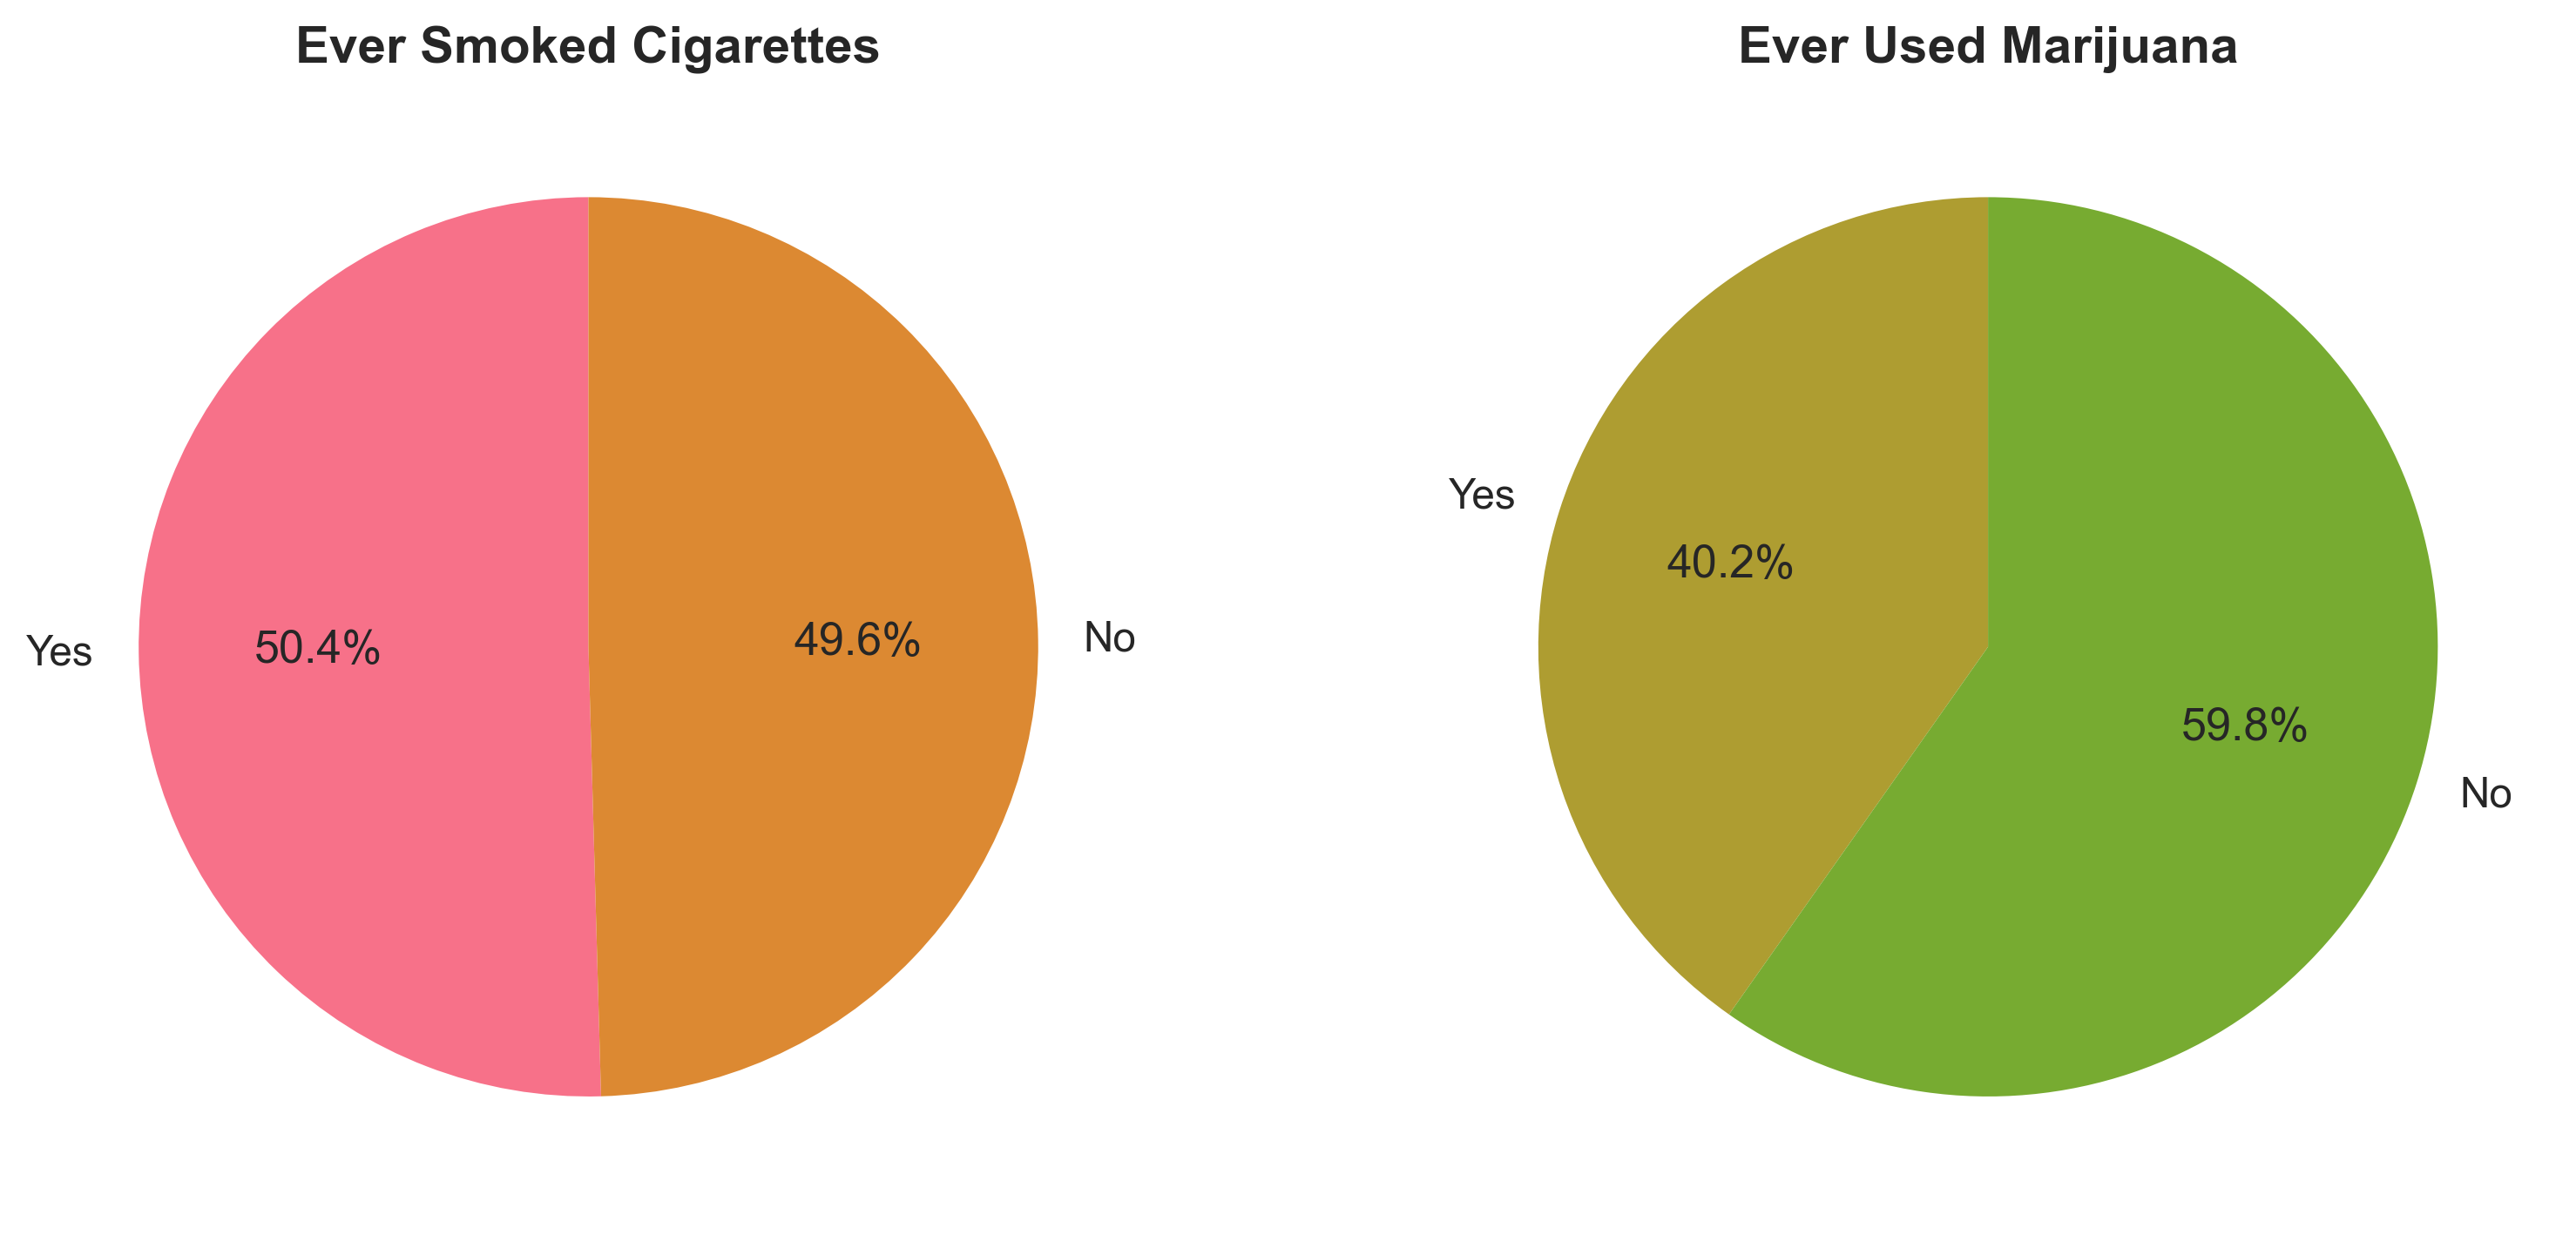
\includegraphics[width=\columnwidth]{figures/fig1_prevalence.png}}
\caption{Lifetime prevalence of cigarette and marijuana use among U.S. population aged 12 and older (N=55,268).}
\label{fig:prevalence}
\end{figure}

The near-even split for cigarette use suggests that cigarette experimentation is remarkably common in the U.S. population. The somewhat lower prevalence of marijuana use indicates that while substantial, marijuana experimentation is less universal than cigarette experimentation.

\subsubsection{Age of Initiation}

Figure \ref{fig:age_init} displays the distribution of ages at which respondents first tried cigarettes and marijuana. For cigarette smoking, the mean age of initiation is 15.5 years (median = 15.0 years), with the distribution showing a pronounced peak during middle to late adolescence. The majority of initiation occurs between ages 12 and 18, with relatively few individuals initiating cigarette use in their twenties or later.

\begin{figure}[htbp]
\centerline{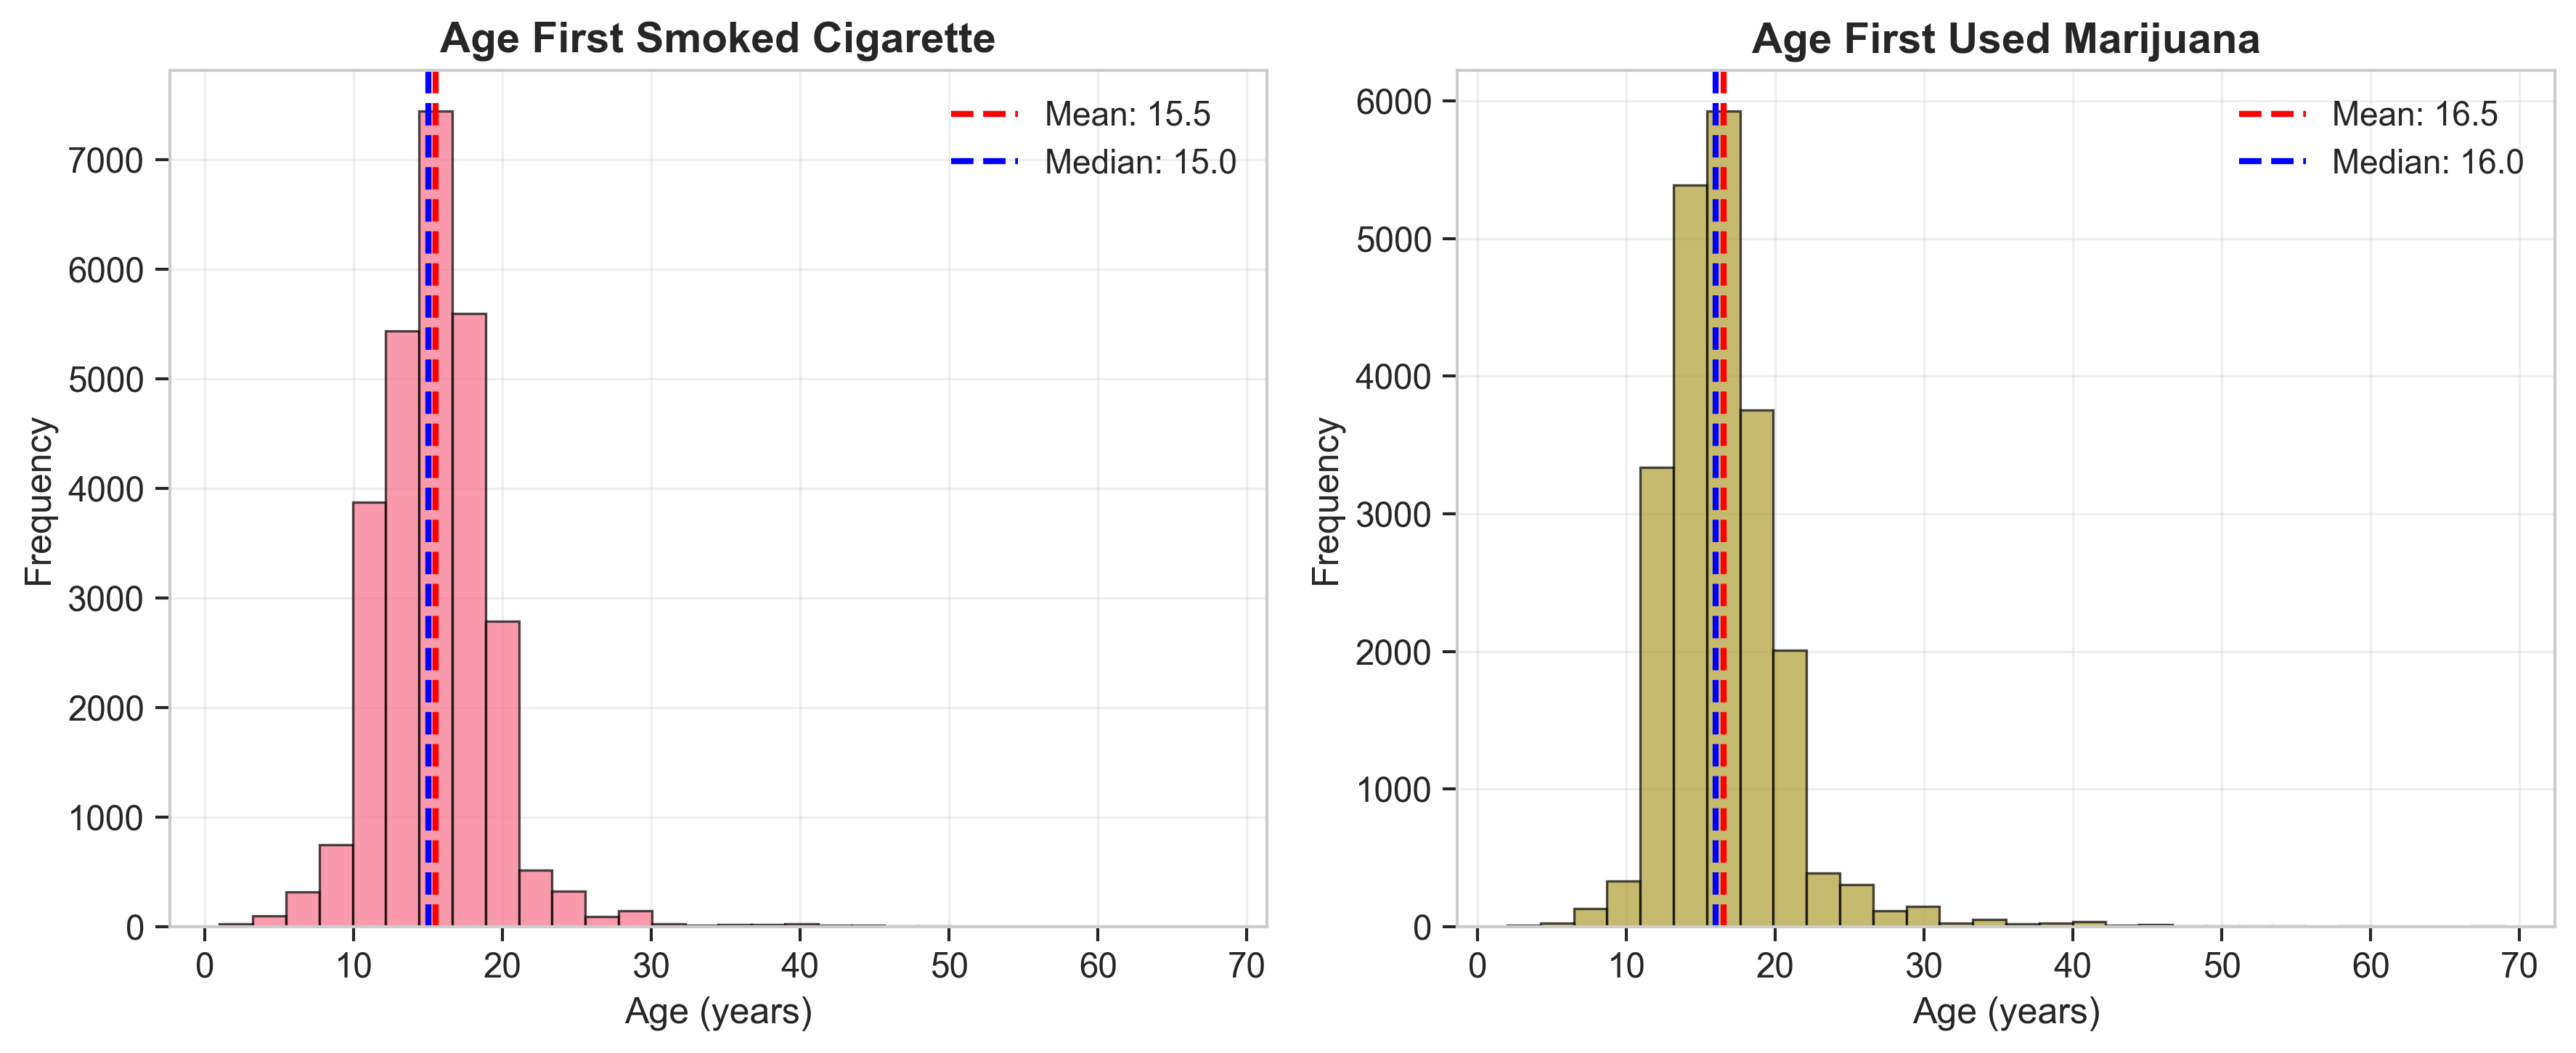
\includegraphics[width=\columnwidth]{figures/fig2_age_initiation.png}}
\caption{Distribution of age at first use for cigarettes and marijuana among ever users.}
\label{fig:age_init}
\end{figure}

For marijuana use, the mean age of initiation is 16.5 years (median = 16.0 years), slightly older than for cigarettes. The marijuana initiation distribution also peaks during adolescence but shows a more gradual decline into early adulthood, suggesting that marijuana initiation continues at meaningful rates into the late teens and early twenties.

These findings underscore the critical importance of school-based prevention programs and early intervention strategies. The slightly later typical age of marijuana initiation compared to cigarettes suggests that prevention efforts for marijuana might need to extend into late adolescence and early adulthood.

\subsubsection{Recent Use Patterns}

Figure \ref{fig:recent_use} illustrates patterns of recent substance use. Among cigarette smokers who used in the past 30 days, the distribution of use days shows considerable variation, with notable peaks at daily use (30 days) and occasional use patterns. This bimodal pattern suggests two distinct user populations: daily smokers and occasional/social smokers.

\begin{figure}[htbp]
\centerline{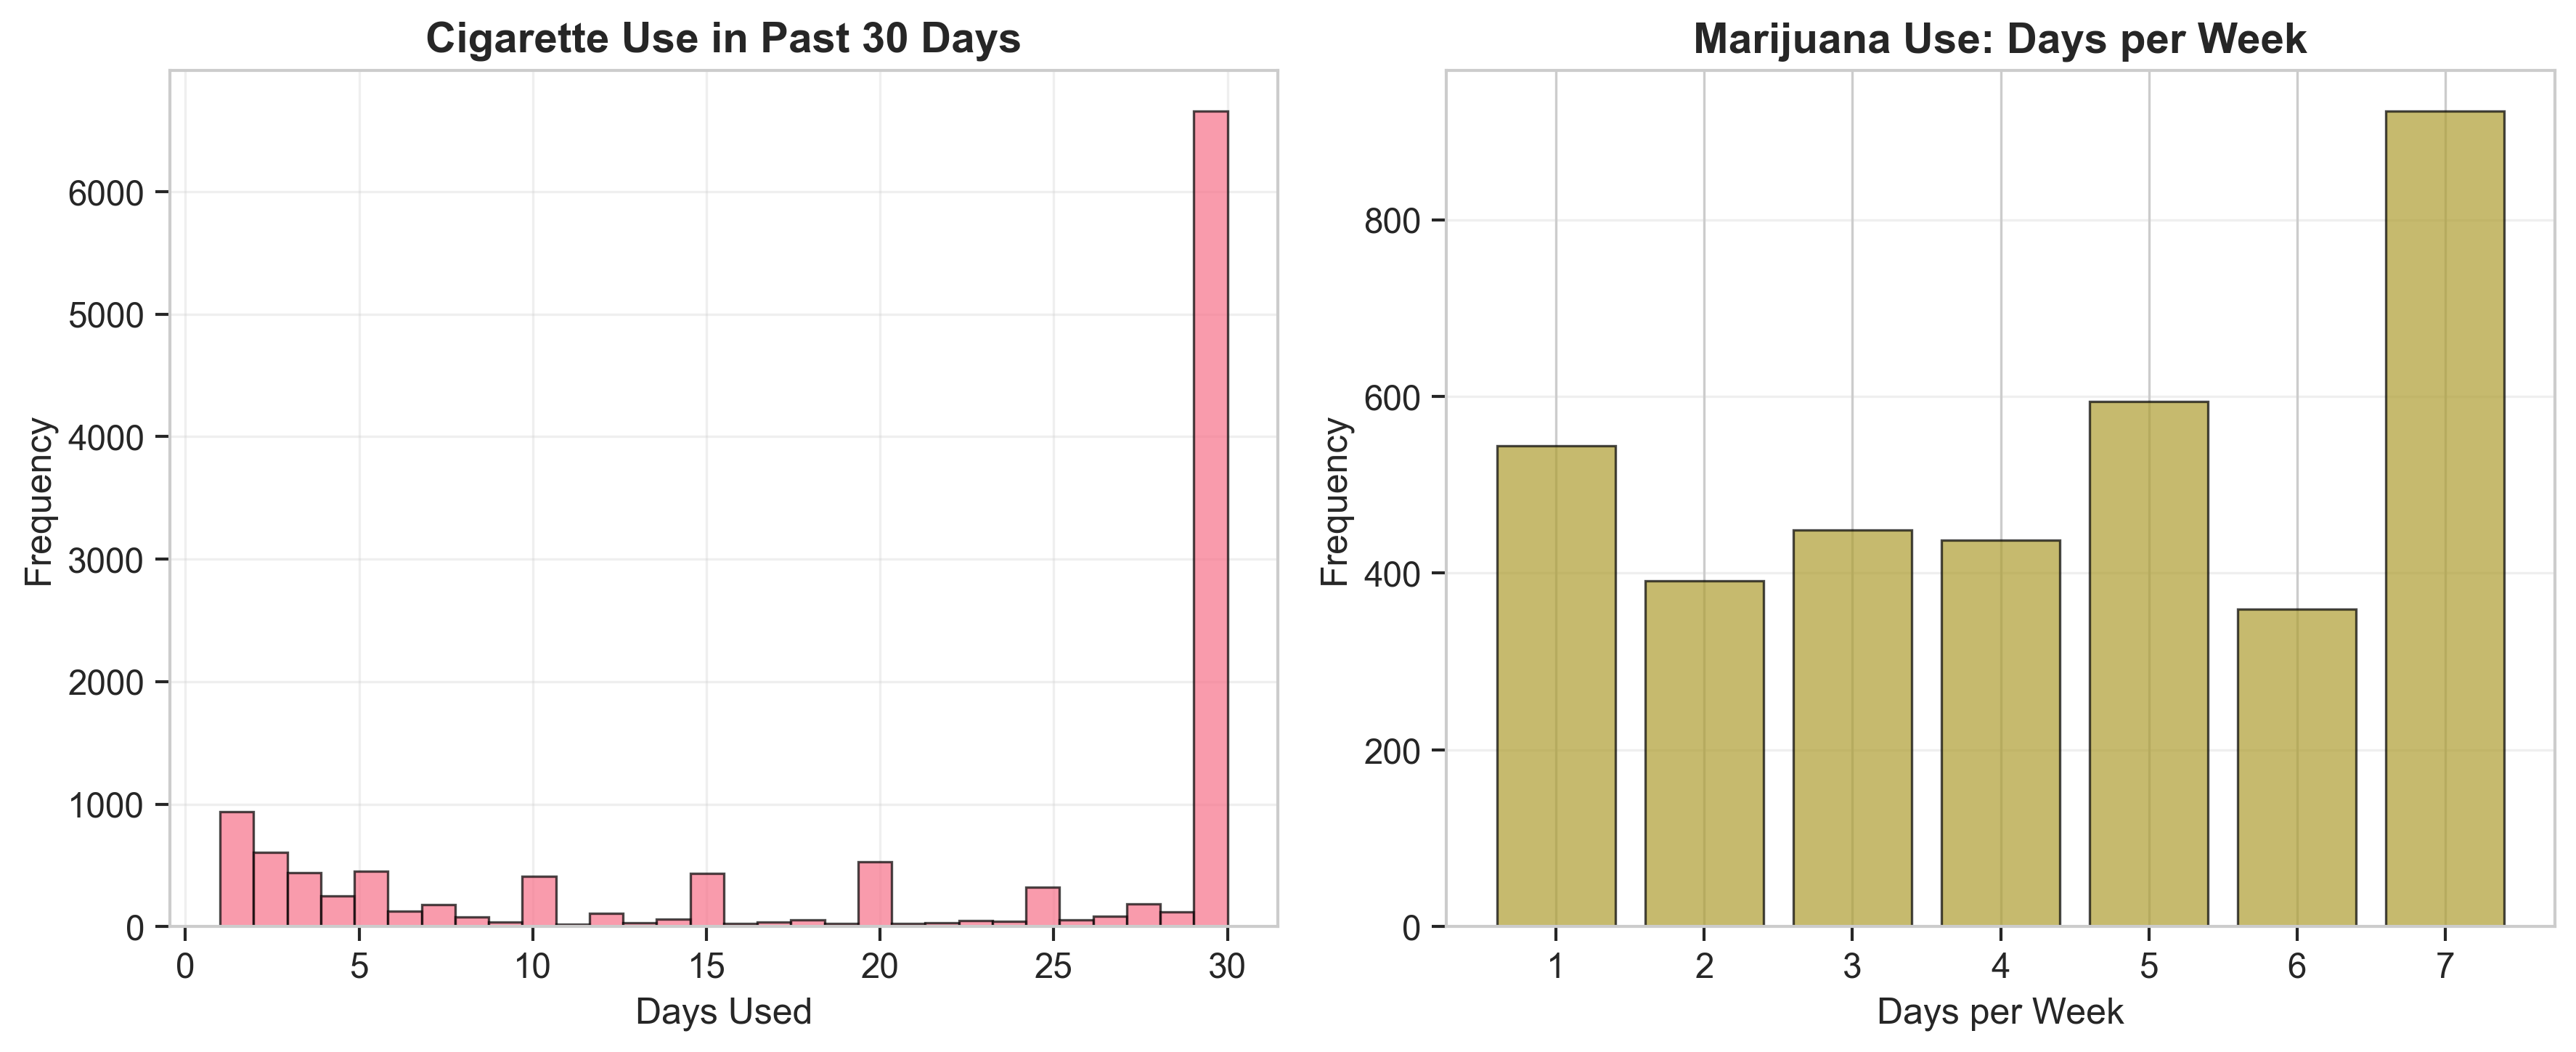
\includegraphics[width=\columnwidth]{figures/fig3_recent_use.png}}
\caption{Recent use patterns: days of cigarette use in past 30 days and days per week of marijuana use in past 12 months.}
\label{fig:recent_use}
\end{figure}

For marijuana use, the frequency distribution measured in days per week over the past 12 months shows that daily or near-daily use (7 days per week) is most common among regular users, followed by weekend use patterns (1-2 days per week). This pattern suggests that among those who use marijuana regularly, daily use is particularly common, which may indicate dependence or habitual use patterns.

\subsubsection{Risk Perception}

Figure \ref{fig:risk} presents respondents' perceptions of risk associated with substance use and related behaviors. For cigarette smoking (1+ pack per day), the overwhelming majority (66.9\%) perceive "great risk," with an additional 24.0\% perceiving "moderate risk." Only a small minority perceive slight or no risk from heavy cigarette smoking. This indicates that public health messaging about the dangers of cigarette smoking has been largely successful in shaping risk perceptions.

\begin{figure}[htbp]
\centerline{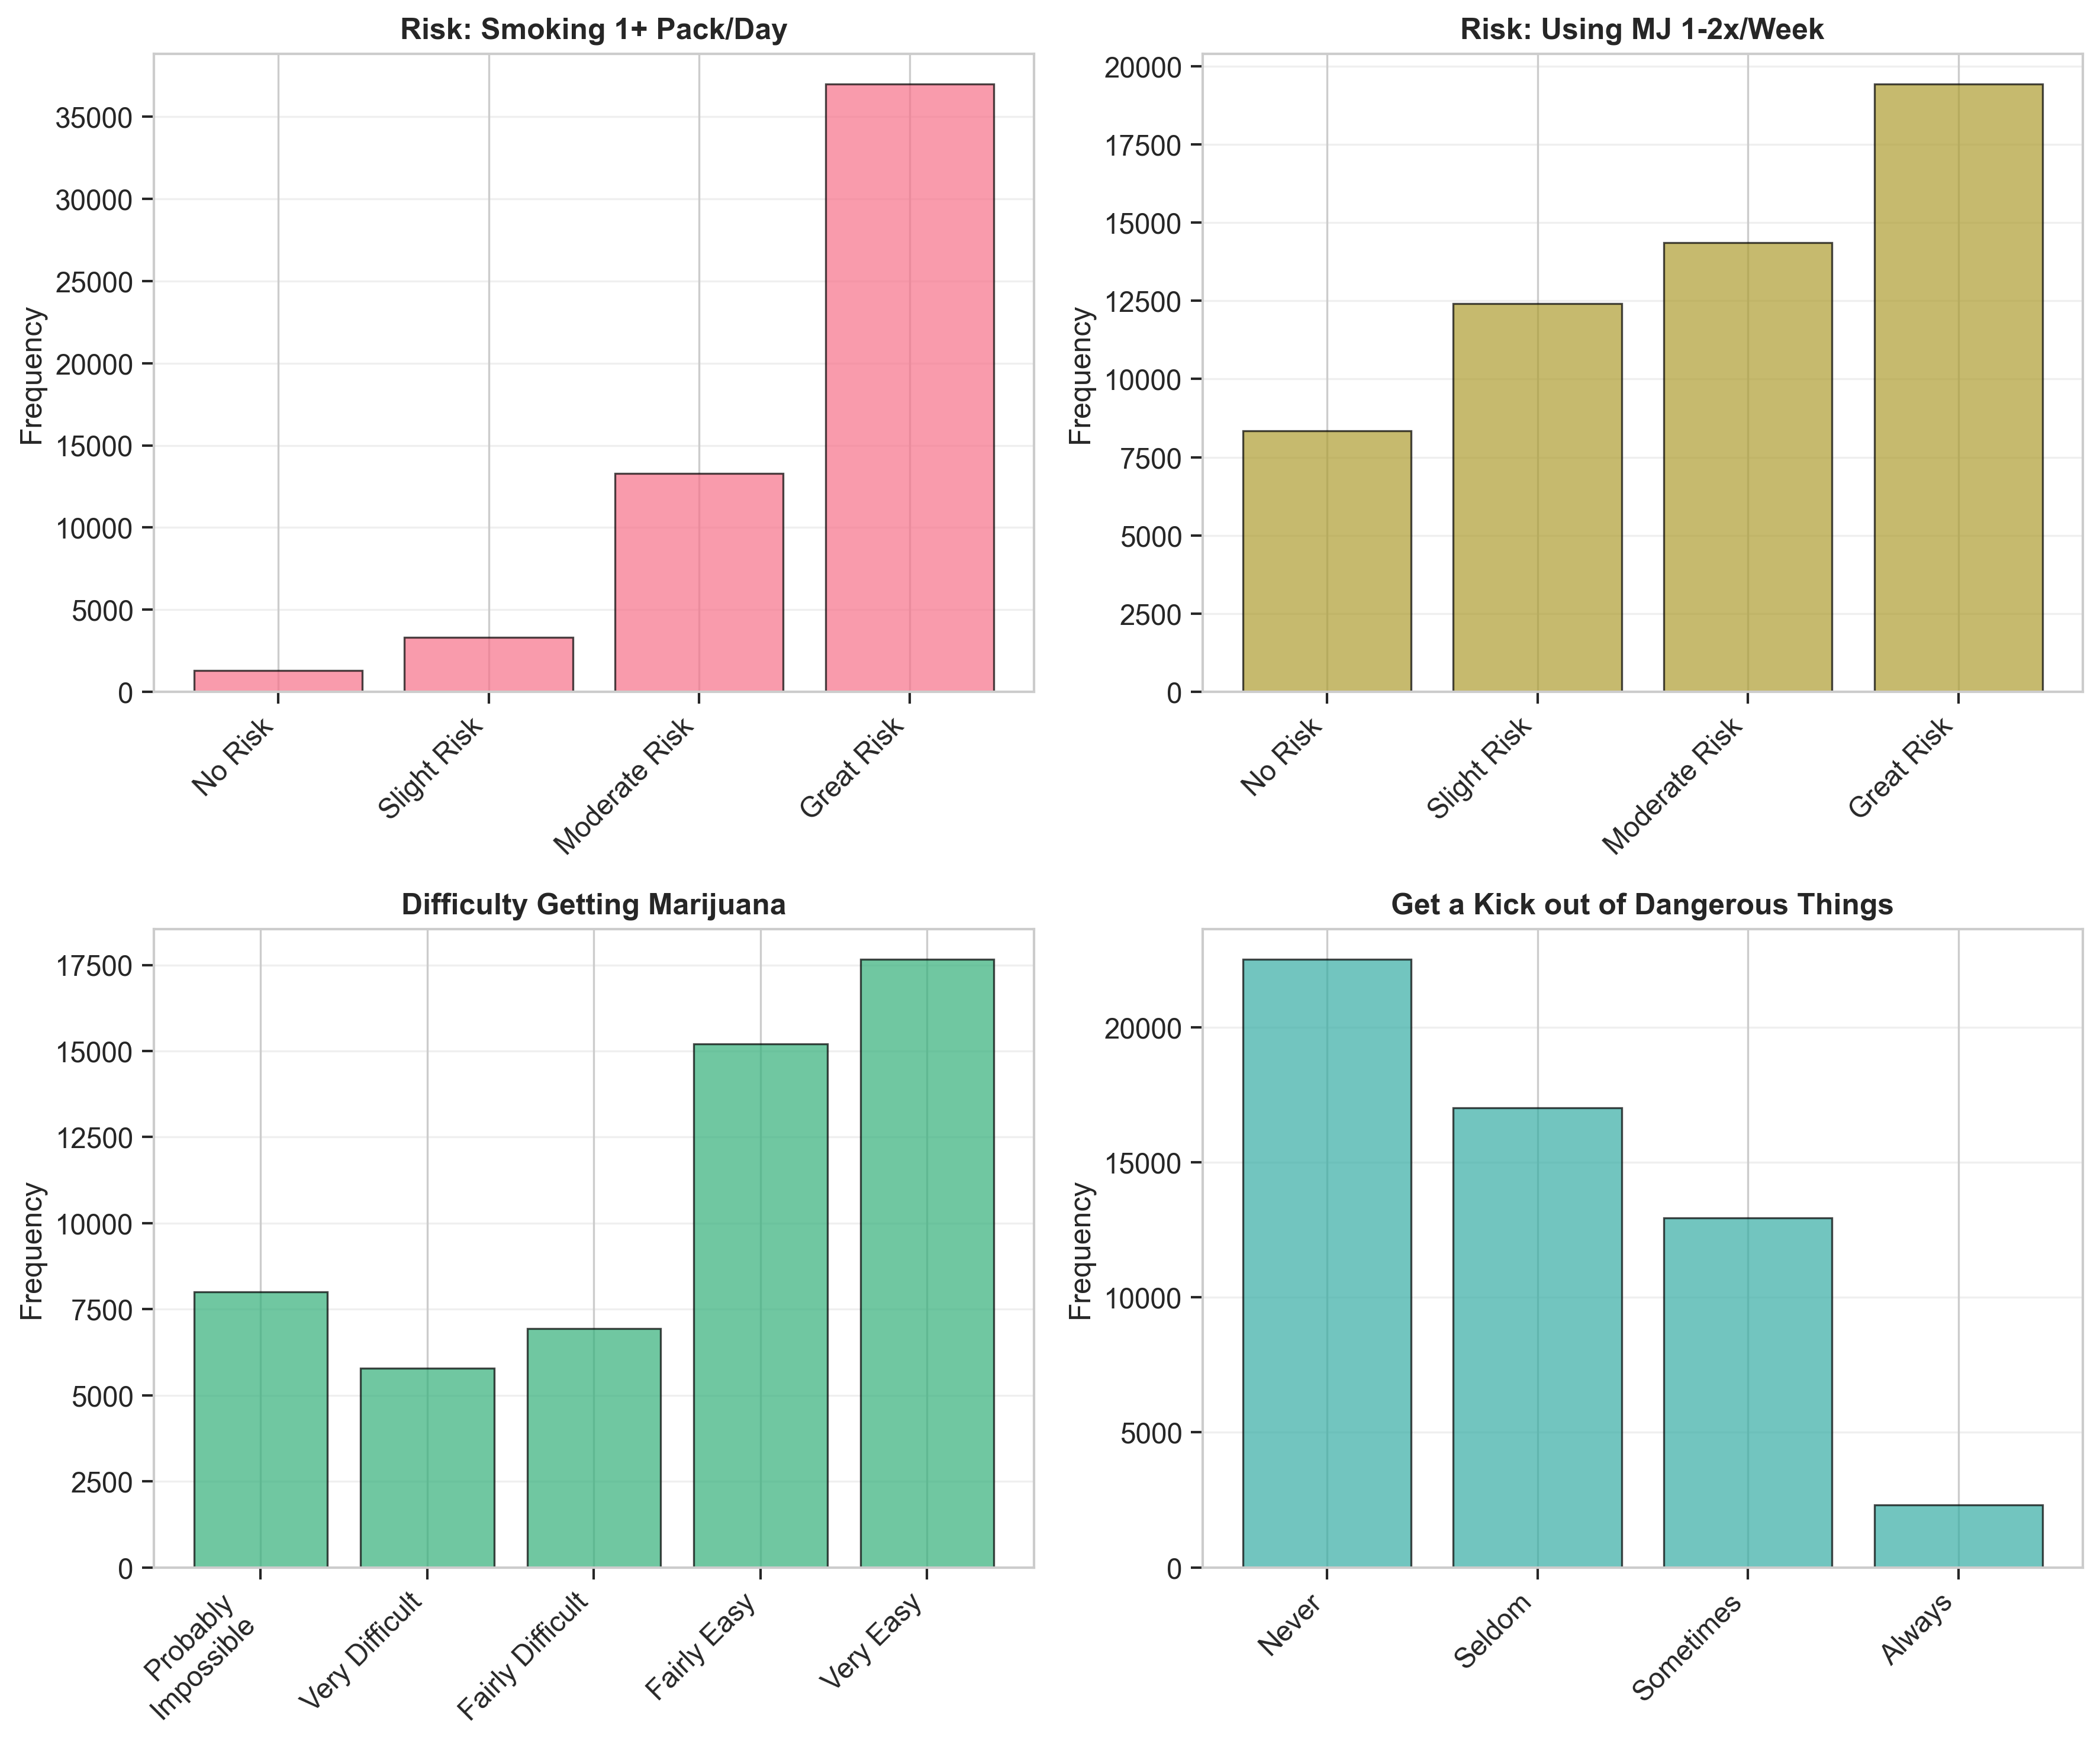
\includegraphics[width=\columnwidth]{figures/fig4_risk_perception.png}}
\caption{Risk perception patterns for cigarette and marijuana use, marijuana accessibility, and risk-taking behavior.}
\label{fig:risk}
\end{figure}

In contrast, risk perceptions for regular marijuana use (1-2 times per week) show greater variation. While 35.2\% perceive "great risk," 26.0\% perceive "moderate risk," 22.5\% perceive "slight risk," and 15.1\% perceive "no risk." This more distributed pattern of risk perception suggests less consensus about the dangers of marijuana use compared to cigarette smoking.

Regarding marijuana accessibility, perceptions are notably divided. A majority of respondents consider marijuana easy to obtain: 31.9\% believe it would be "very easy" and 27.5\% "fairly easy." In contrast, 12.5\% consider it "fairly difficult," 10.5\% "very difficult," and 14.5\% "probably impossible" to obtain. This variation in perceived accessibility may reflect genuine differences in marijuana availability across different communities and social networks.

\subsubsection{Dependence Indicators}

Figure \ref{fig:dependence} shows the distribution of two key nicotine dependence symptoms among cigarette smokers. These items were asked of past-month smokers and are rated on a five-point scale from "not at all true" to "extremely true." For needing cigarettes to feel less irritable, responses show a gradient from "not at all true" (3,575 respondents) to "extremely true" (1,347 respondents), with substantial numbers at each level. This distribution indicates considerable variation in the mood-regulating function of cigarettes among smokers.

\begin{figure}[htbp]
\centerline{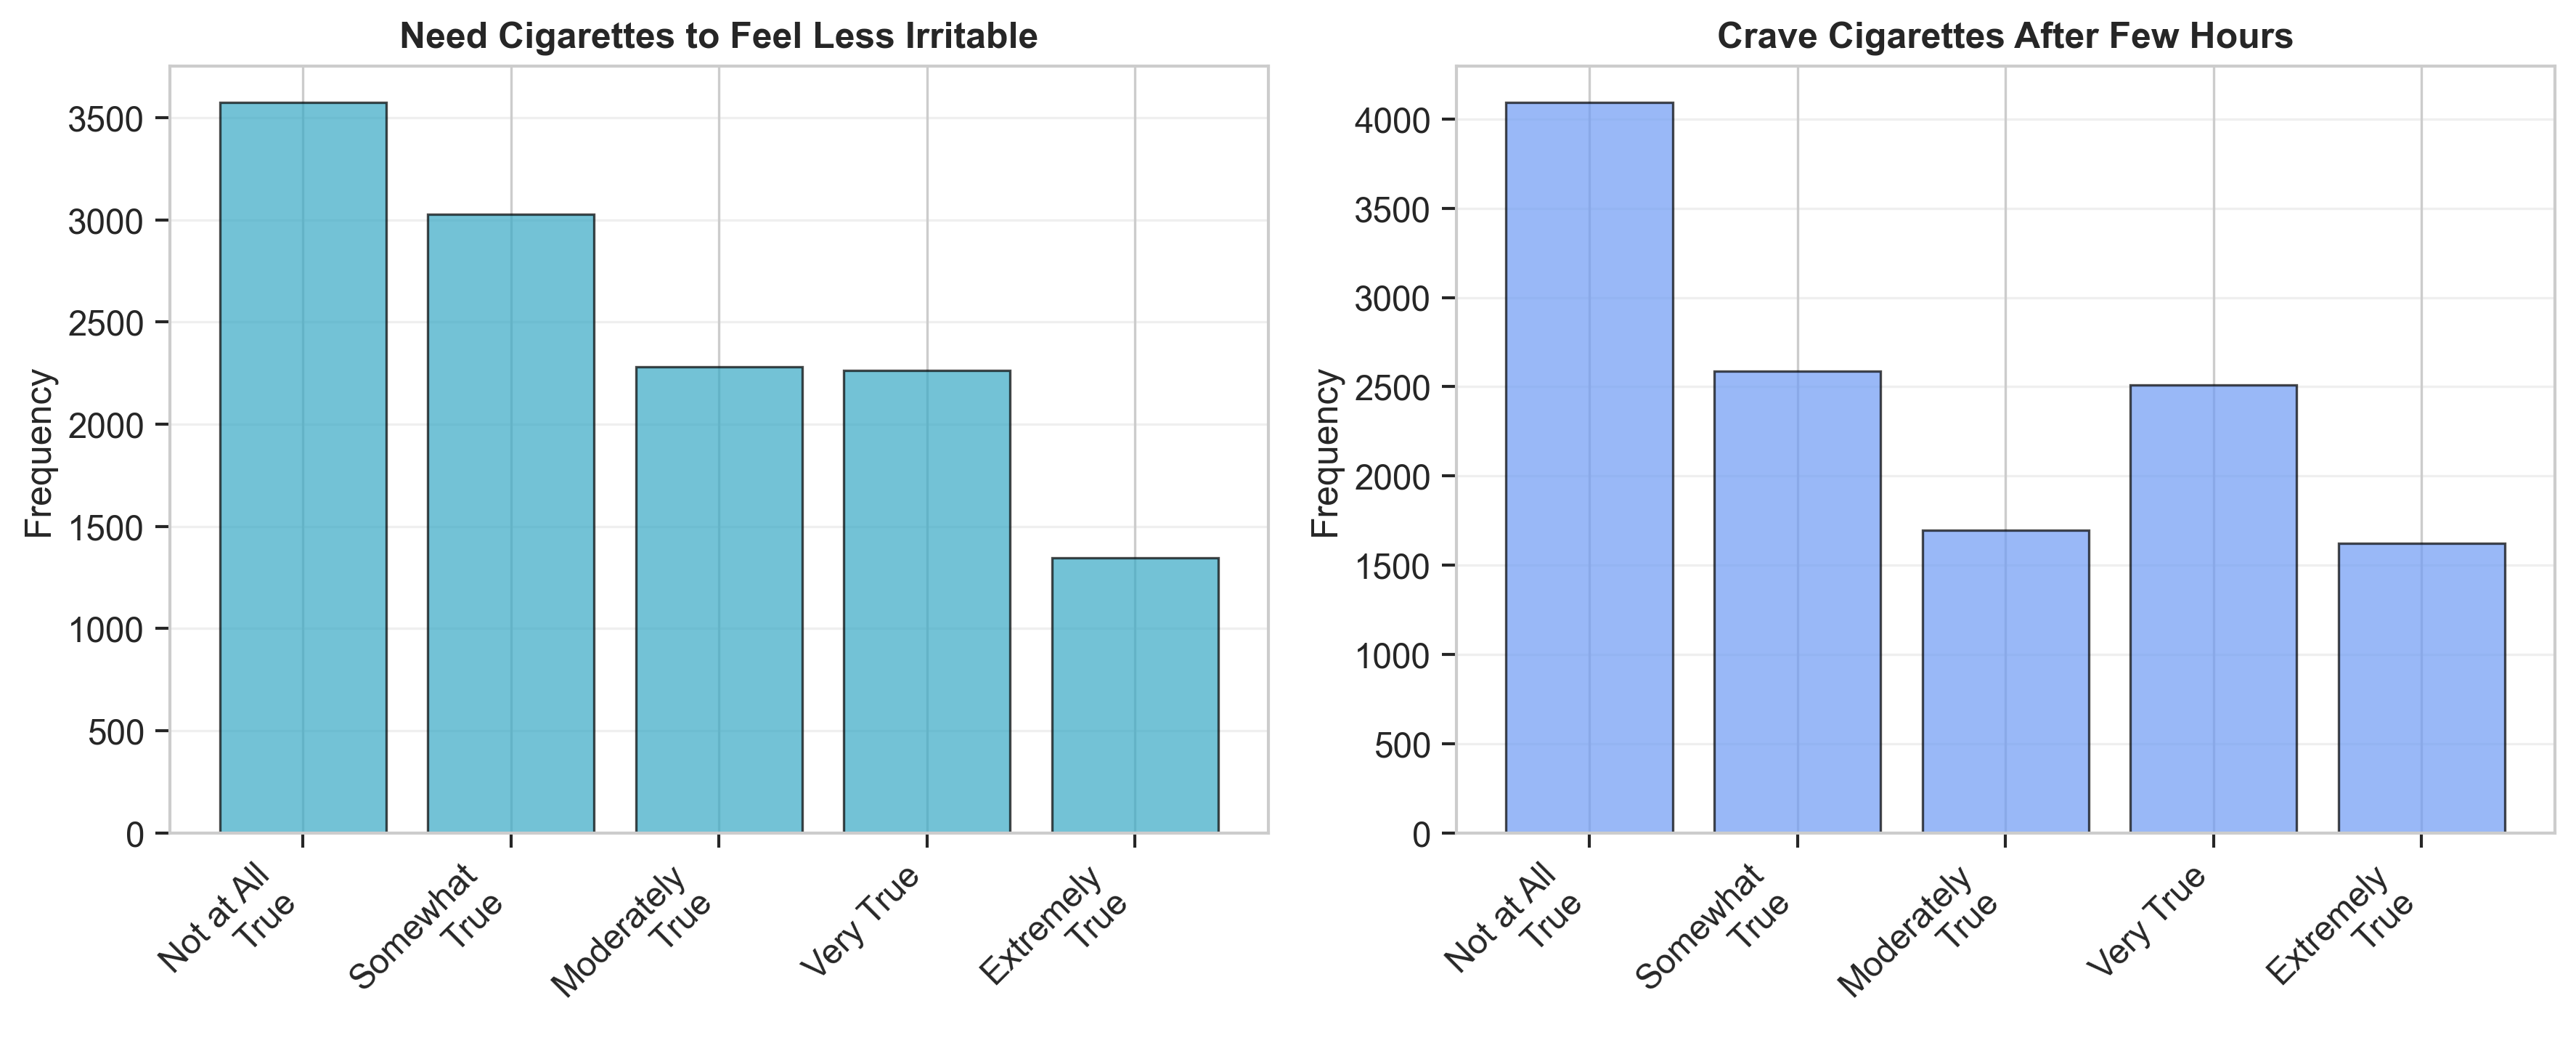
\includegraphics[width=\columnwidth]{figures/fig5_dependence.png}}
\caption{Cigarette dependence indicators: frequency of needing cigarettes to feel less irritable and craving cigarettes after a few hours.}
\label{fig:dependence}
\end{figure}

Craving cigarettes after not smoking for a few hours shows a similar pattern, with 4,093 rating the statement "not at all true" and 1,621 rating it "extremely true." Notably, for both dependence measures, the "not at all true" category has the highest frequency among active smokers, but substantial numbers report experiencing these symptoms at various frequencies, indicating a range of dependence severity.

\subsubsection{Mental Health Indicators}

Figure \ref{fig:mental_health} presents the distribution of three mental health indicators assessed over the past 30 days. These questions were asked only of adults (aged 18 and older); the percentages below are therefore computed among adult respondents who answered each item. For feeling nervous, 35.0\% felt nervous "none of the time," 37.8\% "a little of the time," 20.6\% "some of the time," 4.5\% "most of the time," and 2.1\% "all of the time."

\begin{figure}[htbp]
\centerline{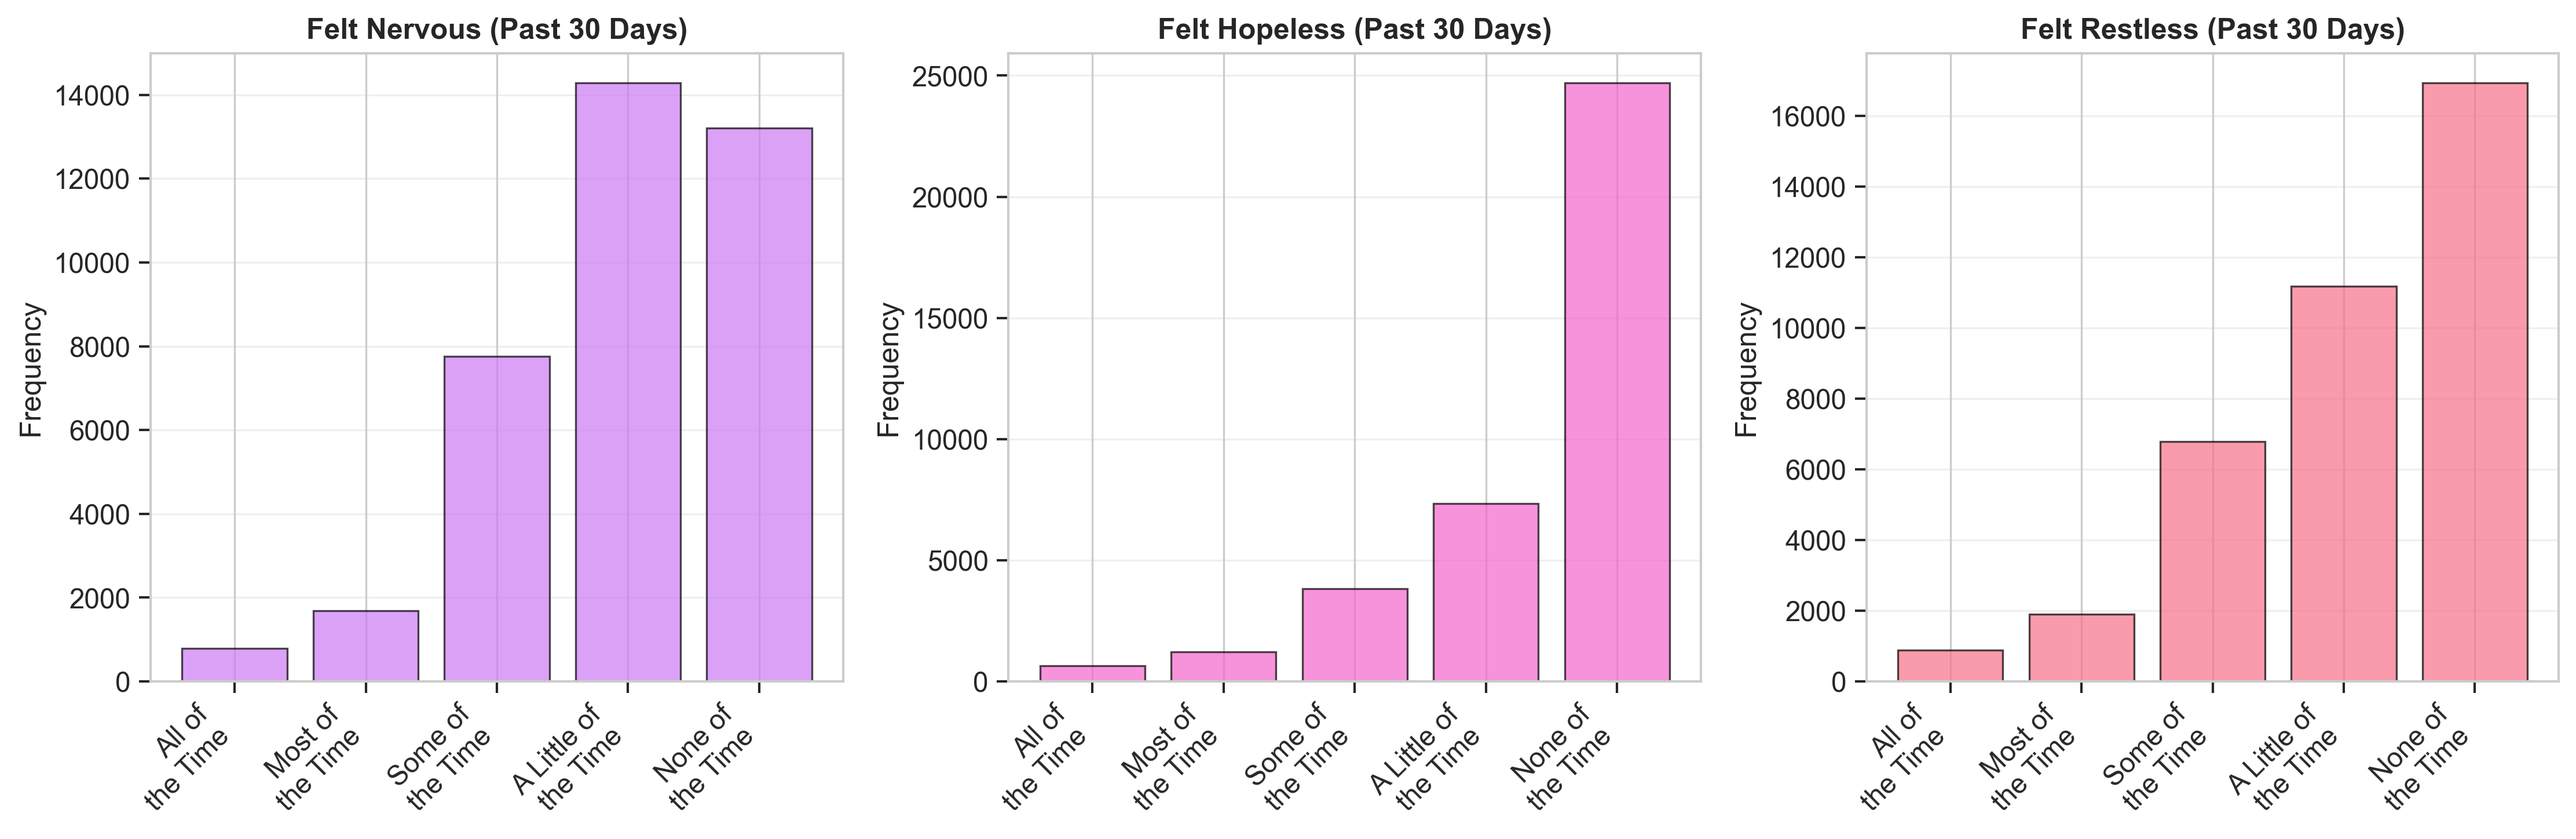
\includegraphics[width=\columnwidth]{figures/fig6_mental_health.png}}
\caption{Mental health indicators: frequency of feeling nervous, hopeless, and restless in the past 30 days.}
\label{fig:mental_health}
\end{figure}

For feeling hopeless, the pattern is more skewed toward lower frequencies, with 65.4\% reporting "none of the time," 19.5\% "a little of the time," 10.1\% "some of the time," 3.2\% "most of the time," and only 1.7\% "all of the time." This suggests that while nervousness is relatively common, feelings of hopelessness are experienced less frequently in the population.

Feeling restless or fidgety falls between the two, with 44.9\% reporting "none of the time," 29.7\% "a little of the time," 18.0\% "some of the time," 5.1\% "most of the time," and 2.4\% "all of the time."

\subsubsection{Demographics}

Figure \ref{fig:demographics} shows the distribution of respondents across age categories and gender-by-age groups. The age distribution shows fairly even representation across the four categories: 12-17 years (31.5\%), 18-25 years (33.7\%), 26-34 years (9.9\%), and 35+ years (24.9\%). The oversampling of younger age groups reflects the survey's emphasis on ages of highest risk for substance use initiation. The gender-by-age indicator (SEXAGE) splits only the two youngest groups by gender (males and females aged 12-17 and 18-25); all respondents aged 26 and older are grouped into a single category.

\begin{figure}[htbp]
\centerline{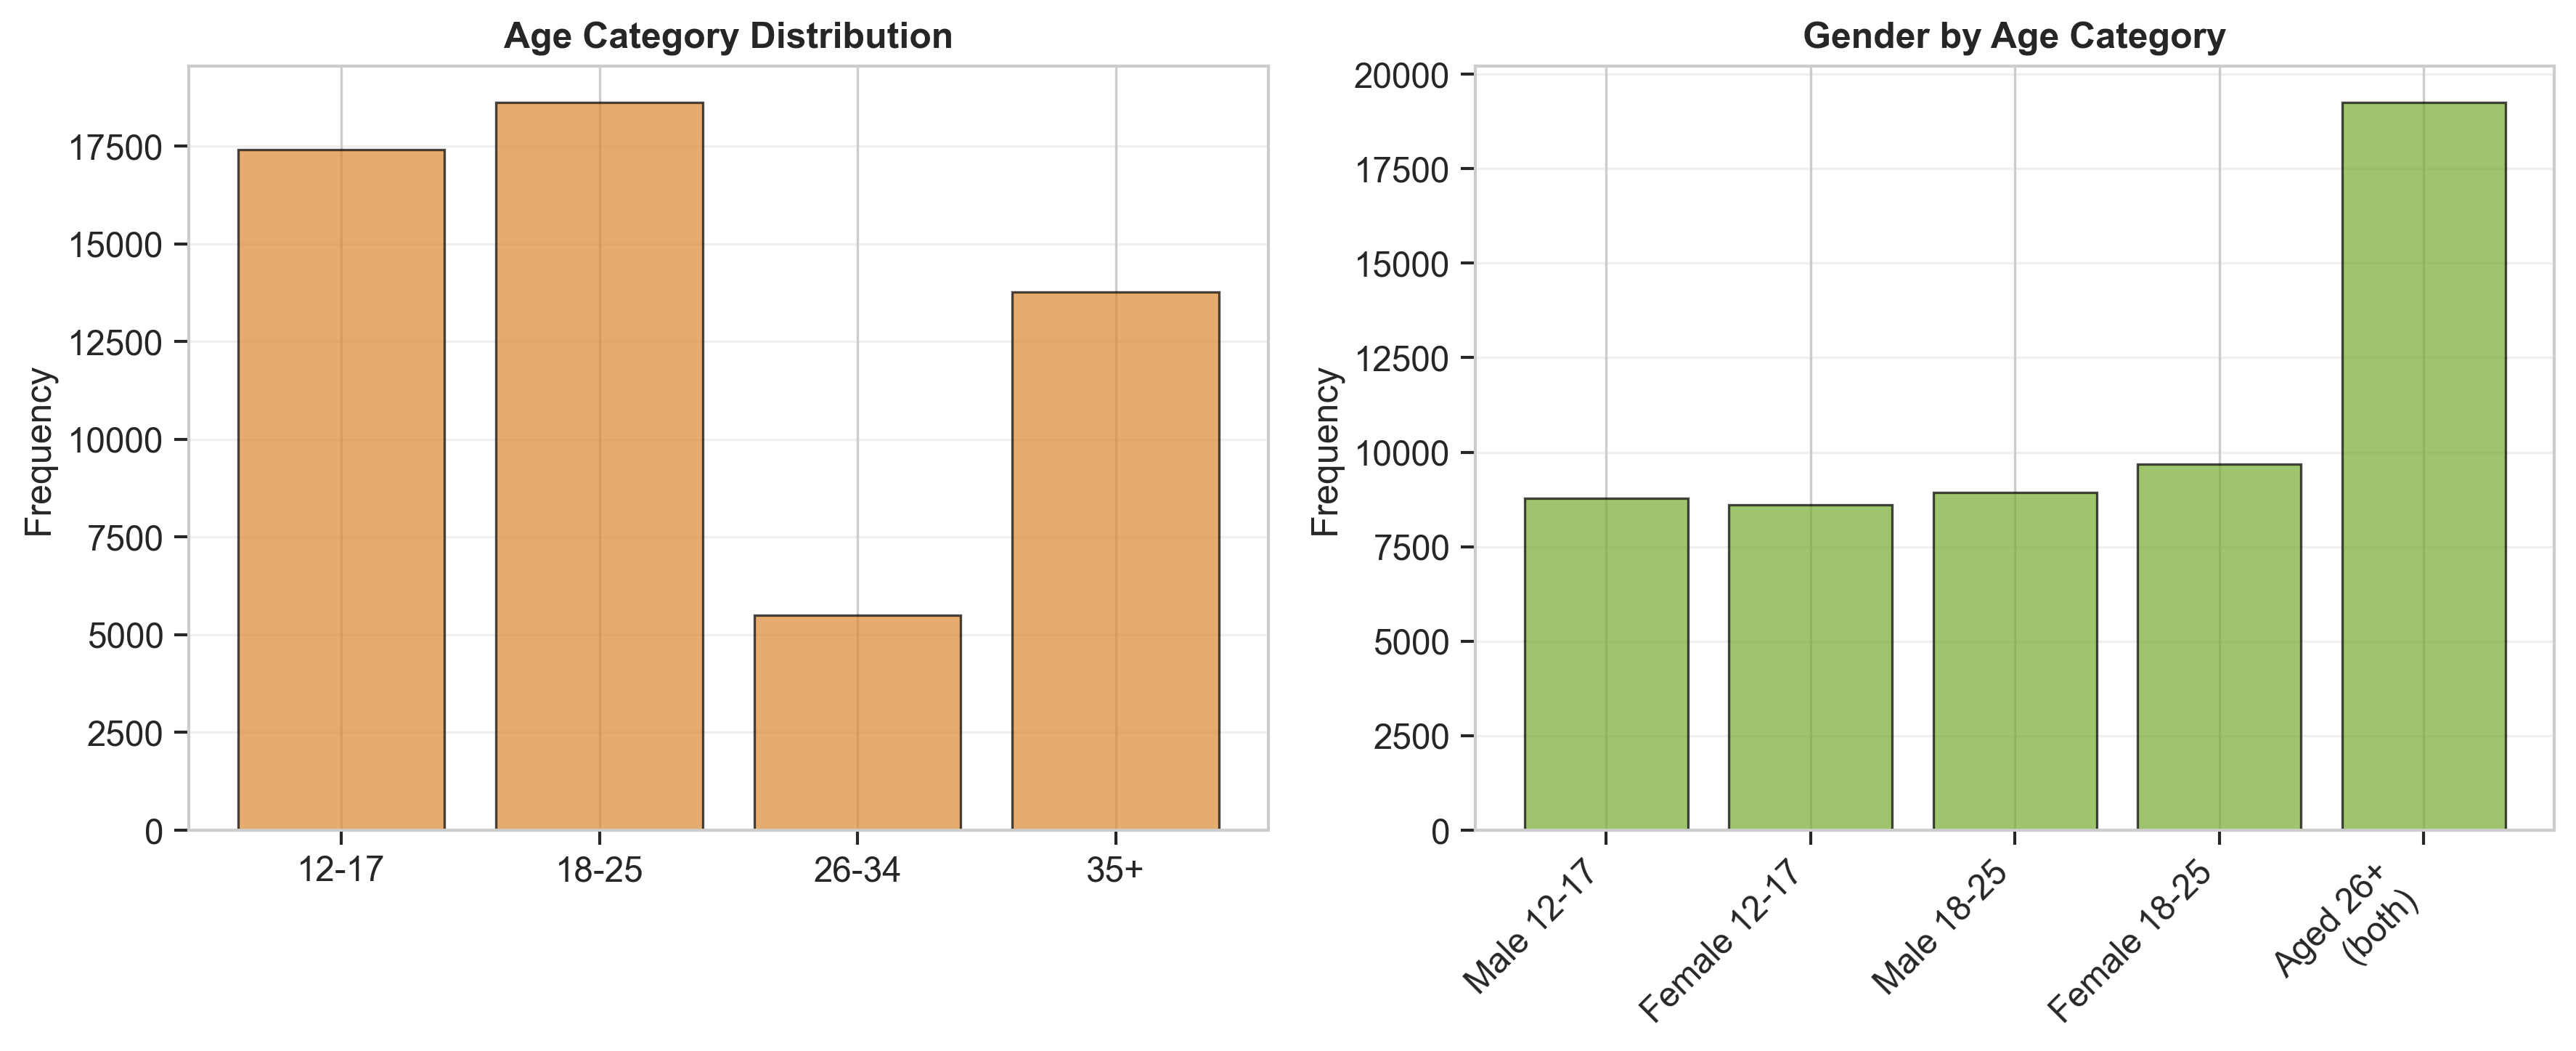
\includegraphics[width=\columnwidth]{figures/fig7_demographics.png}}
\caption{Demographic distribution: age categories and gender by age groups.}
\label{fig:demographics}
\end{figure}

\subsubsection{Marijuana Acquisition}

Figure \ref{fig:acquisition} displays how respondents obtained the marijuana they last used. Among those who reported obtaining marijuana, the most common methods were: receiving it for free or sharing (52.6\%), purchasing it (45.2\%), trading for it (1.2\%), and growing it themselves (1.0\%).

\begin{figure}[htbp]
\centerline{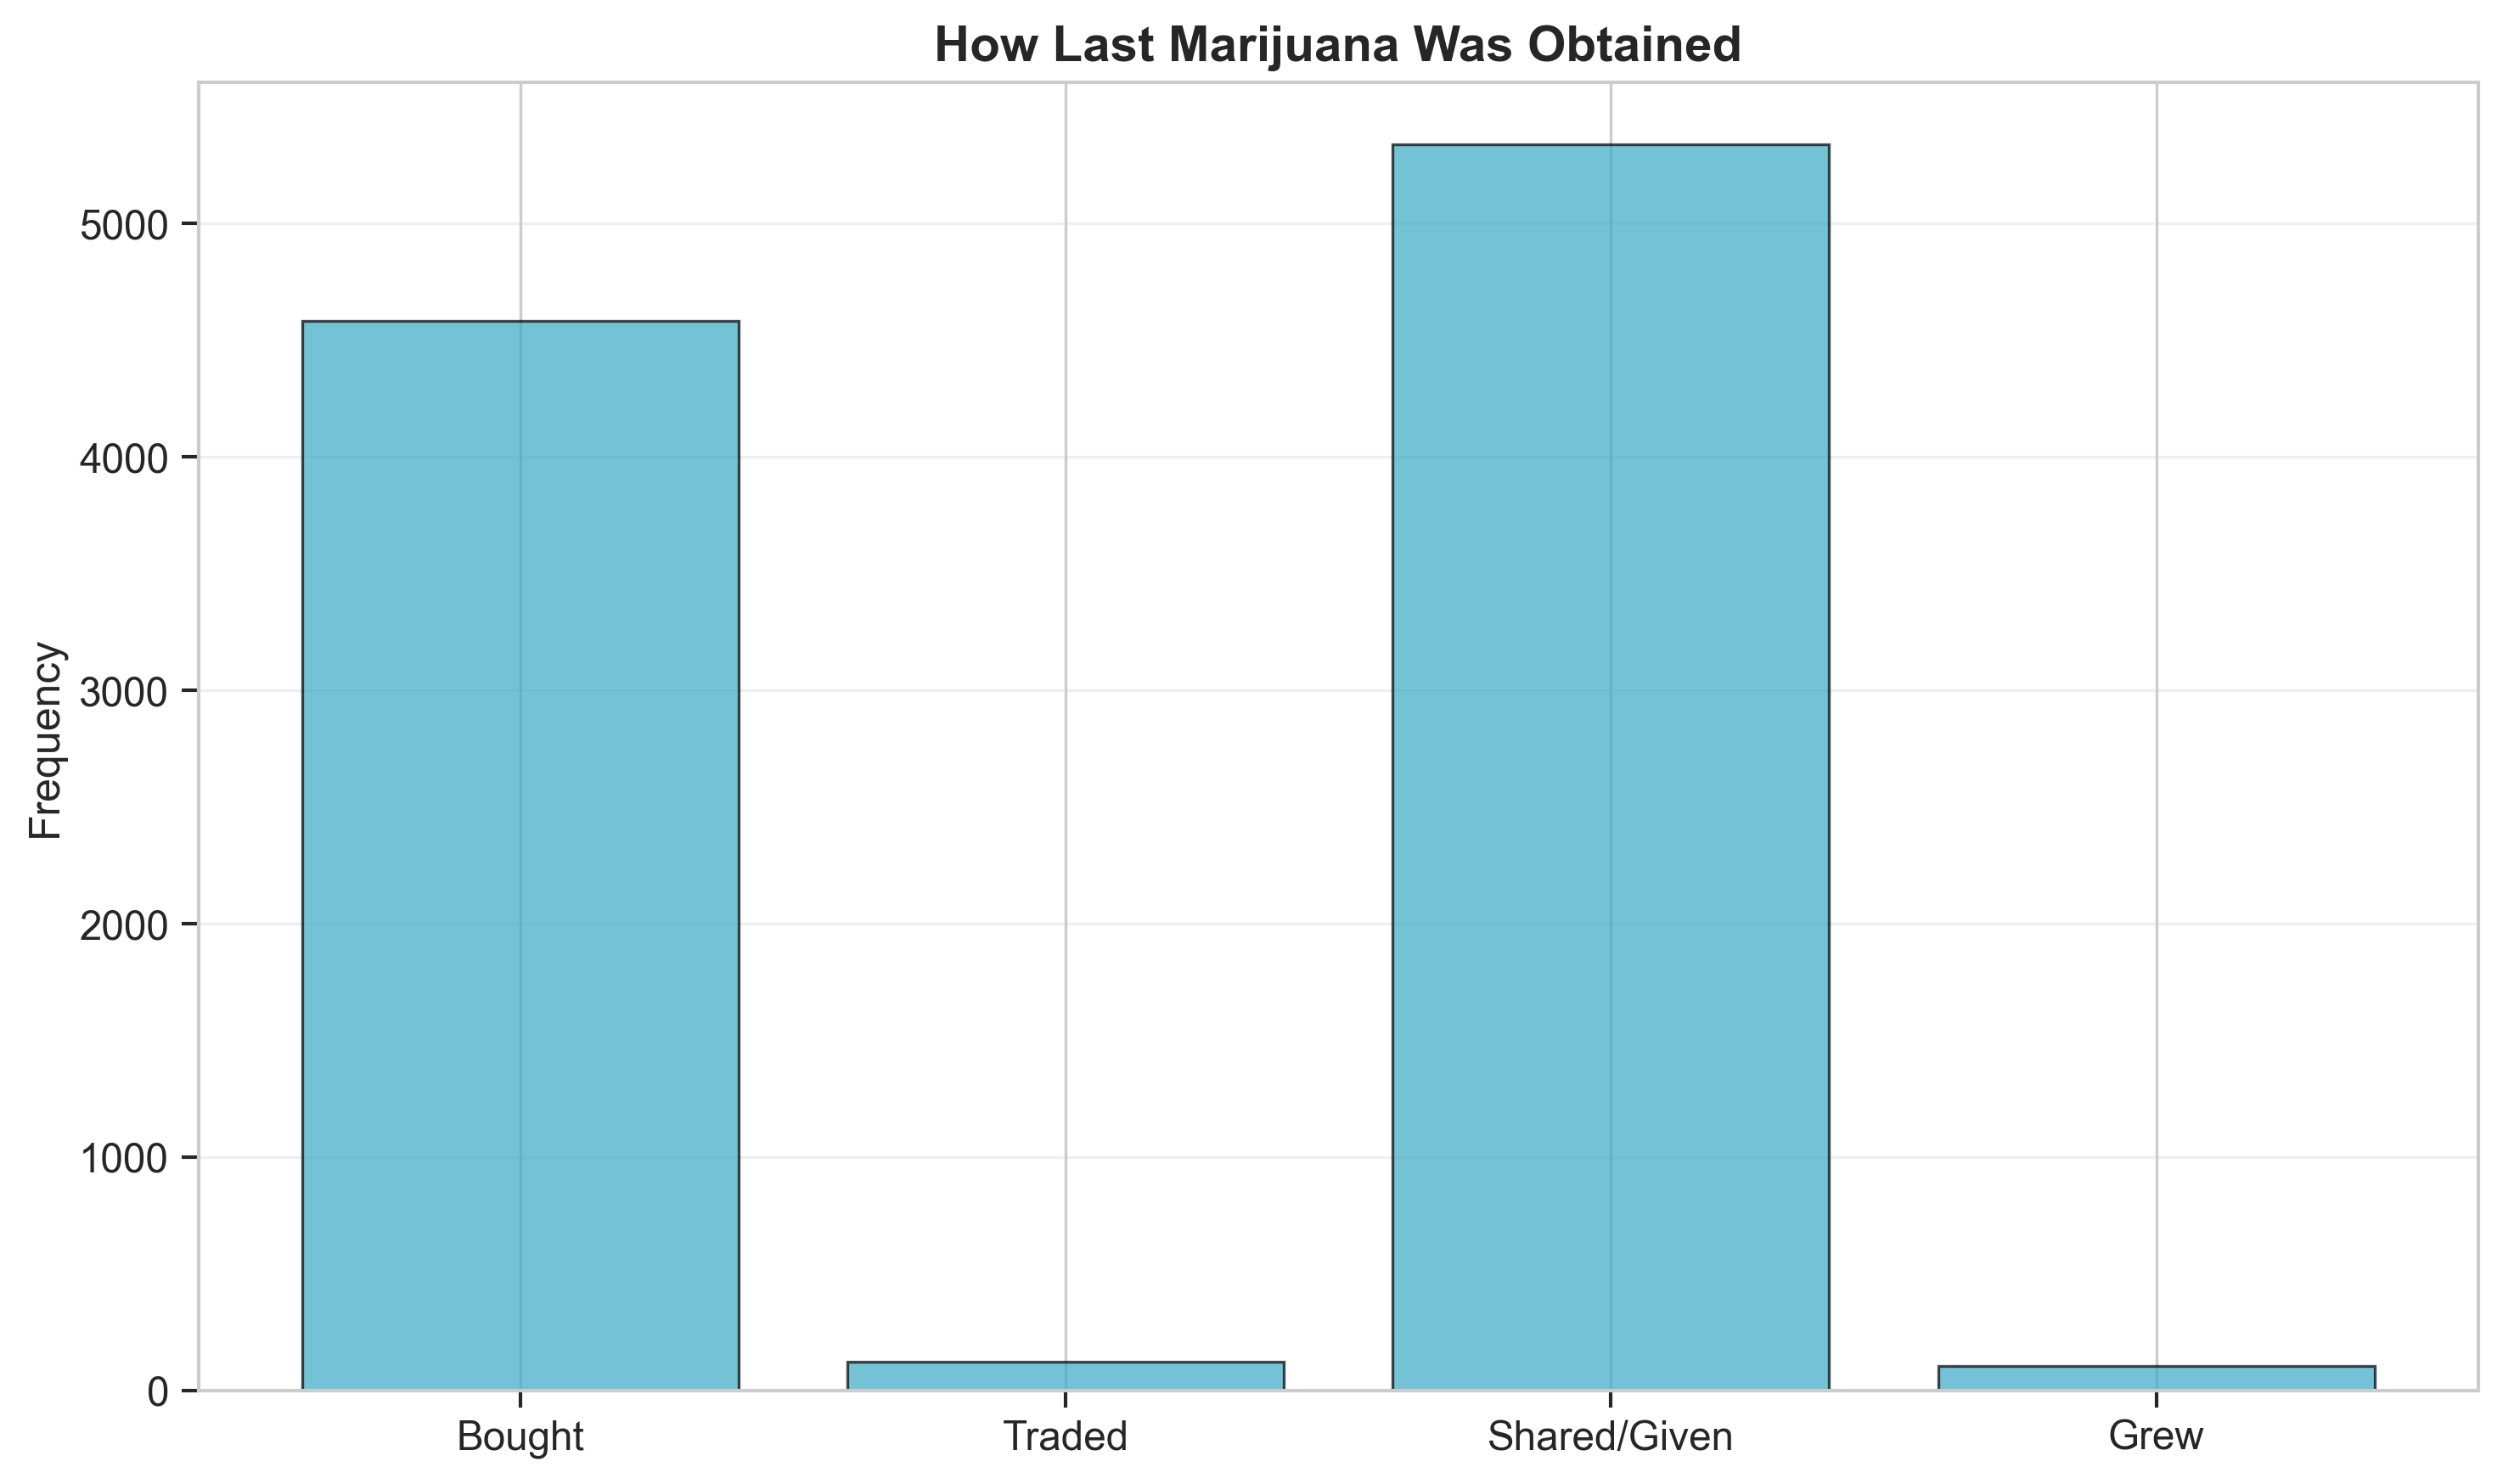
\includegraphics[width=\columnwidth]{figures/fig8_mj_acquisition.png}}
\caption{Methods of obtaining last marijuana used among marijuana users.}
\label{fig:acquisition}
\end{figure}

The predominance of sharing and gifting suggests that social networks play a crucial role in marijuana distribution, particularly for casual or occasional users.

\subsection{Analysis for Answering Research Questions}

\subsubsection{RQ1: Demographic Associations with Substance Use}

Chi-square tests revealed highly significant associations between age group and both cigarette use ($\chi^2$ = 10619.59, df = 3, p $<$ 0.001) and marijuana use ($\chi^2$ = 5564.14, df = 3, p $<$ 0.001). Figure \ref{fig:age_prev} illustrates these dramatic age-related differences.

\begin{figure}[htbp]
\centerline{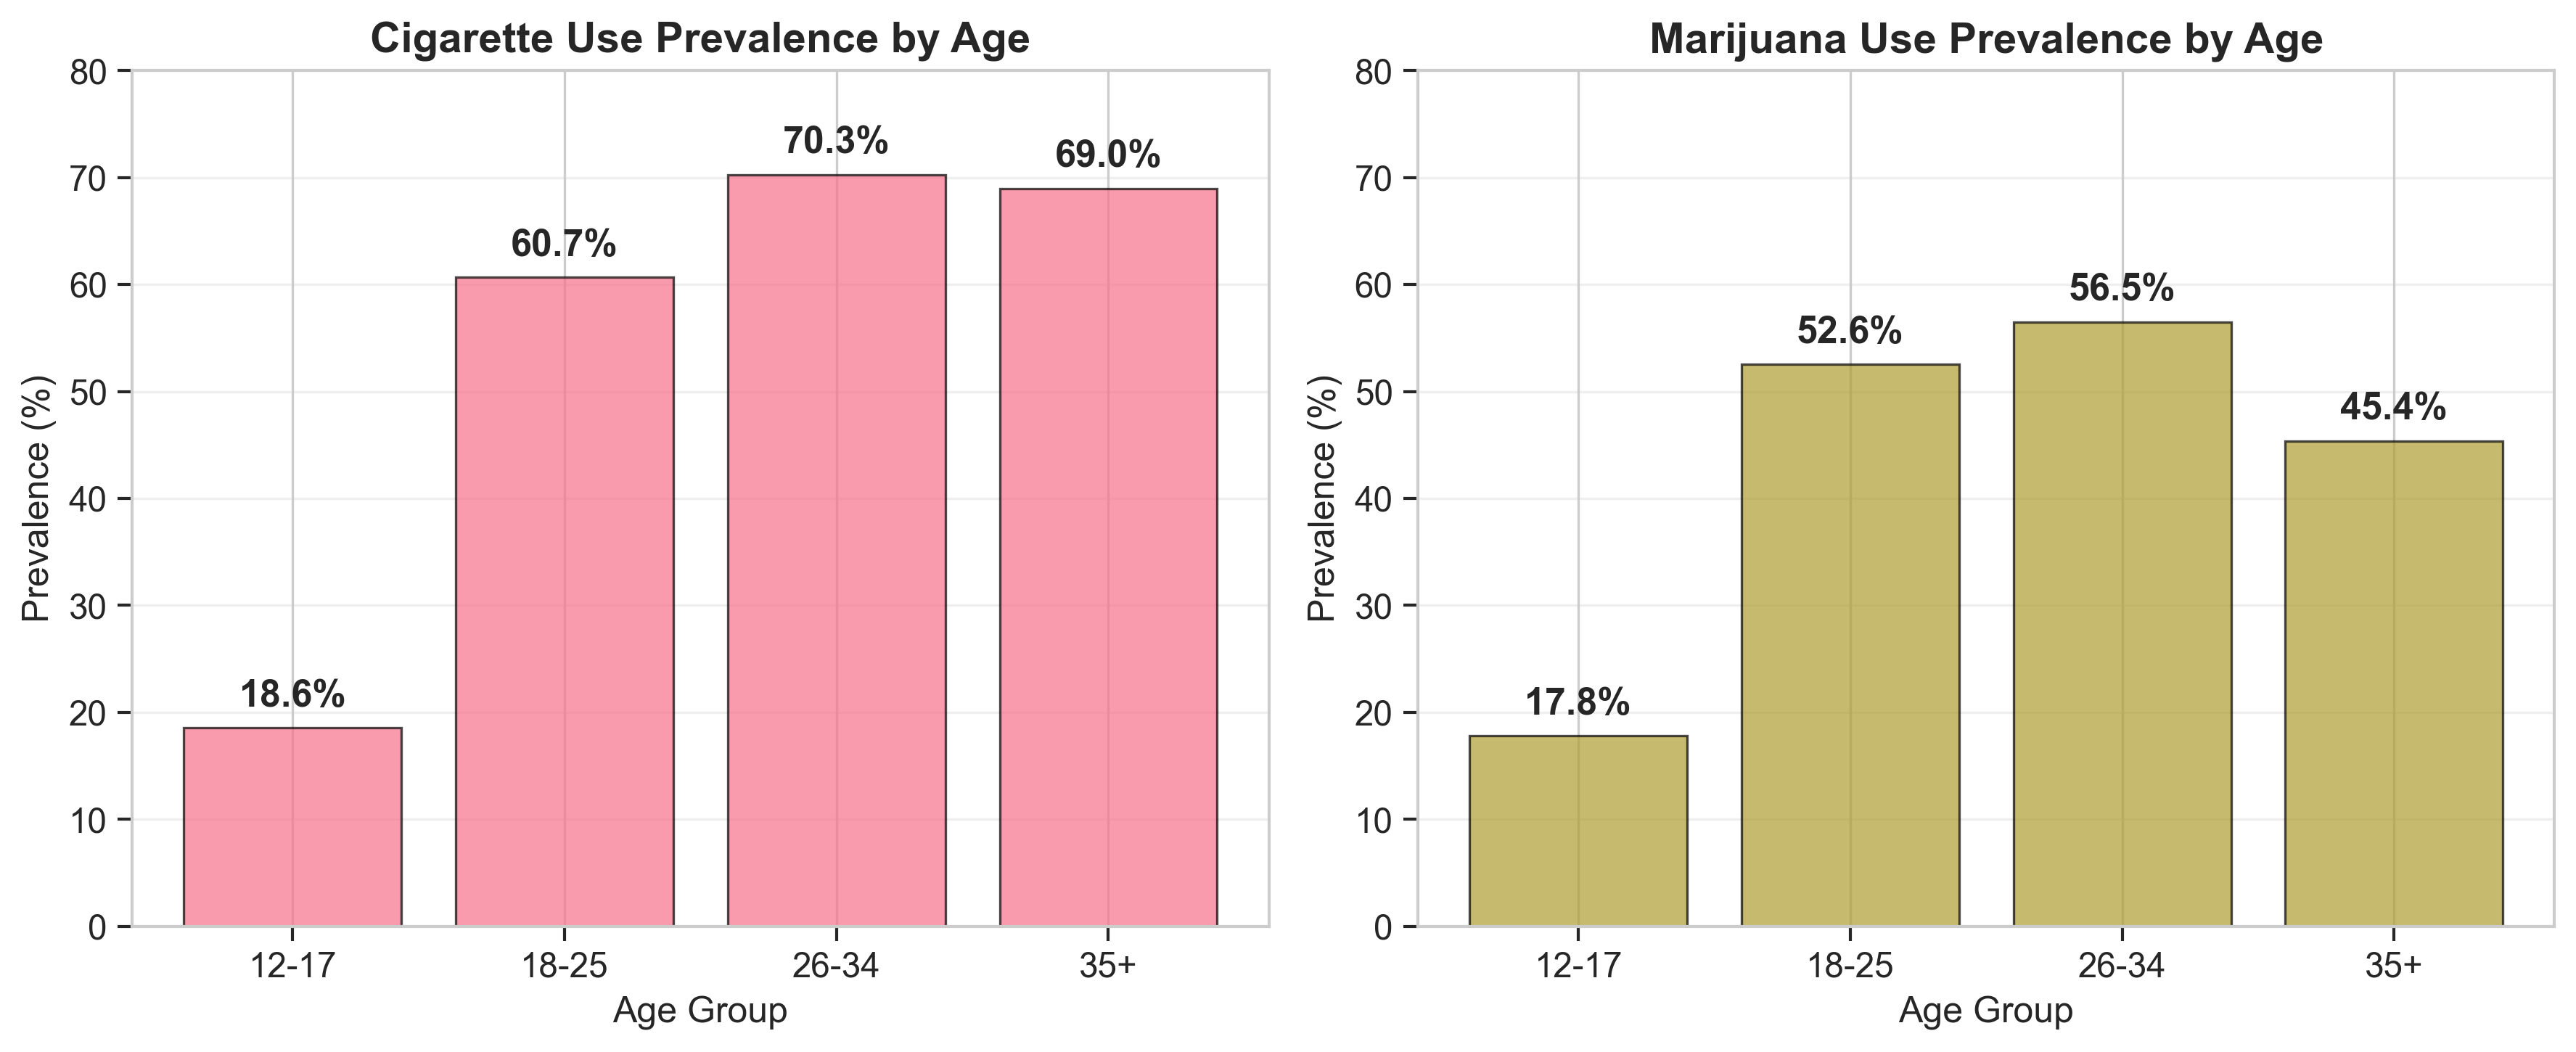
\includegraphics[width=\columnwidth]{figures/fig9_prevalence_by_age.png}}
\caption{Cigarette and marijuana use prevalence by age group, showing dramatic increases from adolescence to young adulthood.}
\label{fig:age_prev}
\end{figure}

For cigarettes, prevalence increases from 18.6\% among 12-17 year-olds to 60.7\% among 18-25 year-olds, then plateaus at approximately 70\% for older age groups. This pattern suggests that most cigarette experimentation occurs during the transition from adolescence to young adulthood, with relatively little new initiation after age 25.

For marijuana, prevalence follows a similar but slightly different pattern, increasing from 17.8\% among 12-17 year-olds to 52.6\% among 18-25 year-olds and 56.5\% among 26-34 year-olds, before declining slightly to 45.4\% among those 35 and older. The decline in older age groups may reflect cohort effects, as marijuana use has become more prevalent in recent decades.

These findings have important implications for prevention efforts. The dramatic increase in use between adolescence and young adulthood suggests that the 18-25 age period is particularly critical for intervention. Programs targeting college students and young adults may be especially important.

\subsubsection{RQ2: Gender Differences in Initiation Age}

Independent samples t-tests revealed significant gender differences in initiation ages for both substances. For cigarettes, males initiated use at a mean age of 15.3 years (SD = 3.7) compared to 15.7 years (SD = 4.0) for females, a difference that was statistically significant (t = -7.97, p $<$ 0.001). For marijuana, males initiated at 16.3 years (SD = 3.9) compared to 16.8 years (SD = 4.2) for females (t = -10.08, p $<$ 0.001).

Figure \ref{fig:gender_init} displays these distributions, showing that while the differences are statistically significant, they are relatively modest in magnitude (approximately 4-6 months earlier for males).

\begin{figure}[htbp]
\centerline{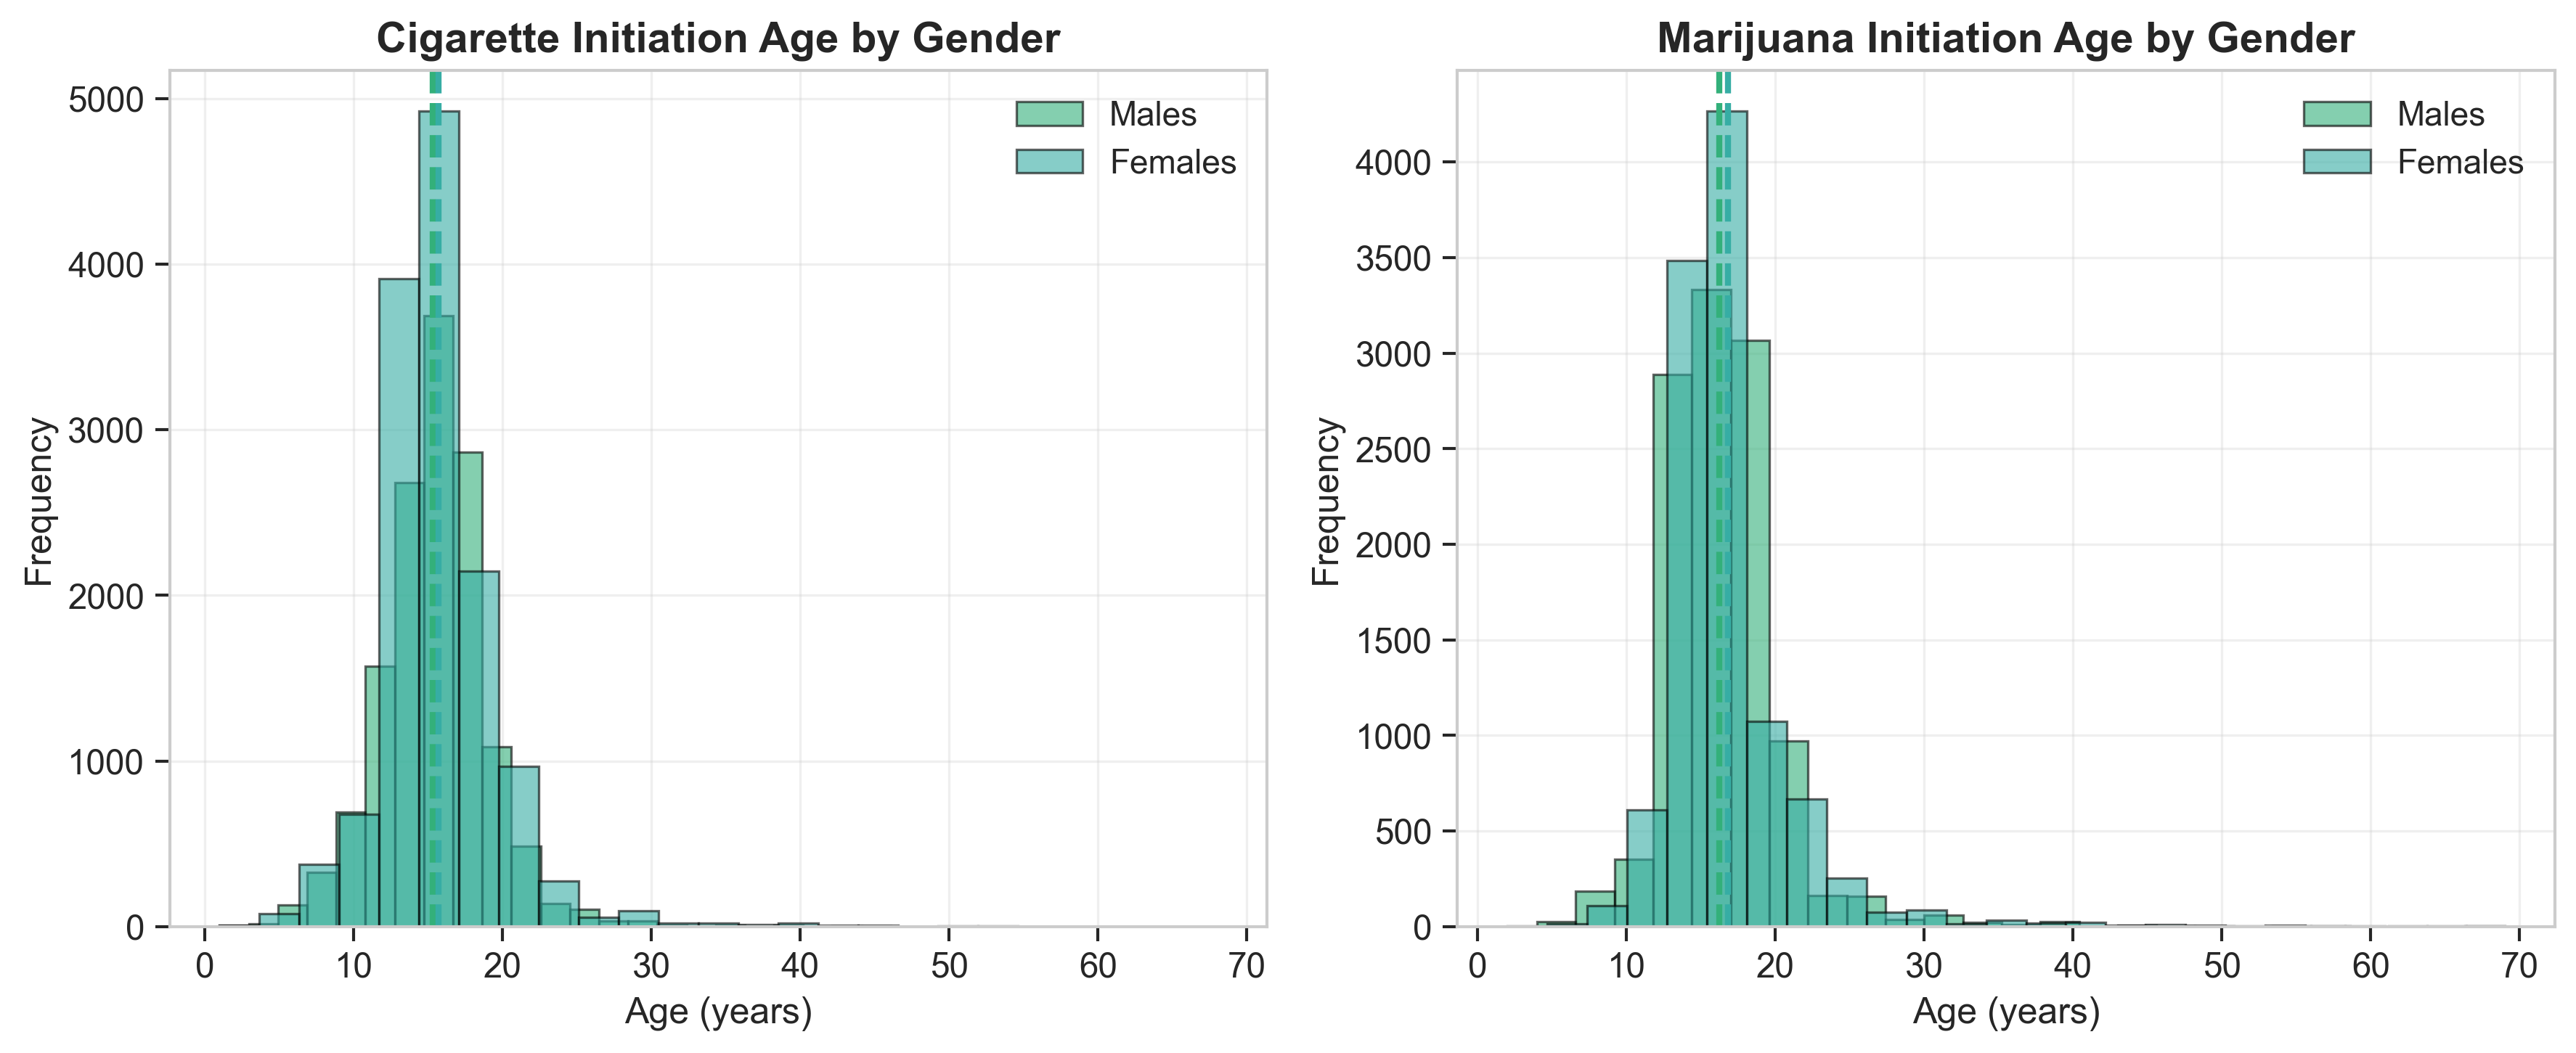
\includegraphics[width=\columnwidth]{figures/fig10_initiation_gender.png}}
\caption{Age of initiation distributions by gender for cigarettes and marijuana, showing earlier initiation among males.}
\label{fig:gender_init}
\end{figure}

Among individuals who used both substances (n=18,544), paired samples t-tests showed that cigarettes were initiated significantly earlier (mean = 15.1 years) than marijuana (mean = 16.4 years), with a mean difference of 1.3 years (t = -43.61, p $<$ 0.001). This consistent pattern of cigarette-first initiation has important implications for gateway theories and prevention sequencing.

\subsubsection{RQ3: Risk Perception and Use Behaviors}

Spearman correlation analyses revealed significant inverse relationships between risk perception and use for both substances. For cigarettes, the correlation was modest (r = -0.081, p $<$ 0.001), while for marijuana the relationship was substantially stronger (r = -0.461, p $<$ 0.001).

Figure \ref{fig:risk_use} illustrates these relationships by comparing risk perception distributions between users and non-users. For cigarettes, users and non-users show relatively similar risk perceptions, with both groups largely recognizing great risk (mean ratings: 3.51 for users vs. 3.62 for non-users on a 1-4 scale). This suggests that cigarette use often occurs despite awareness of risk.

\begin{figure}[htbp]
\centerline{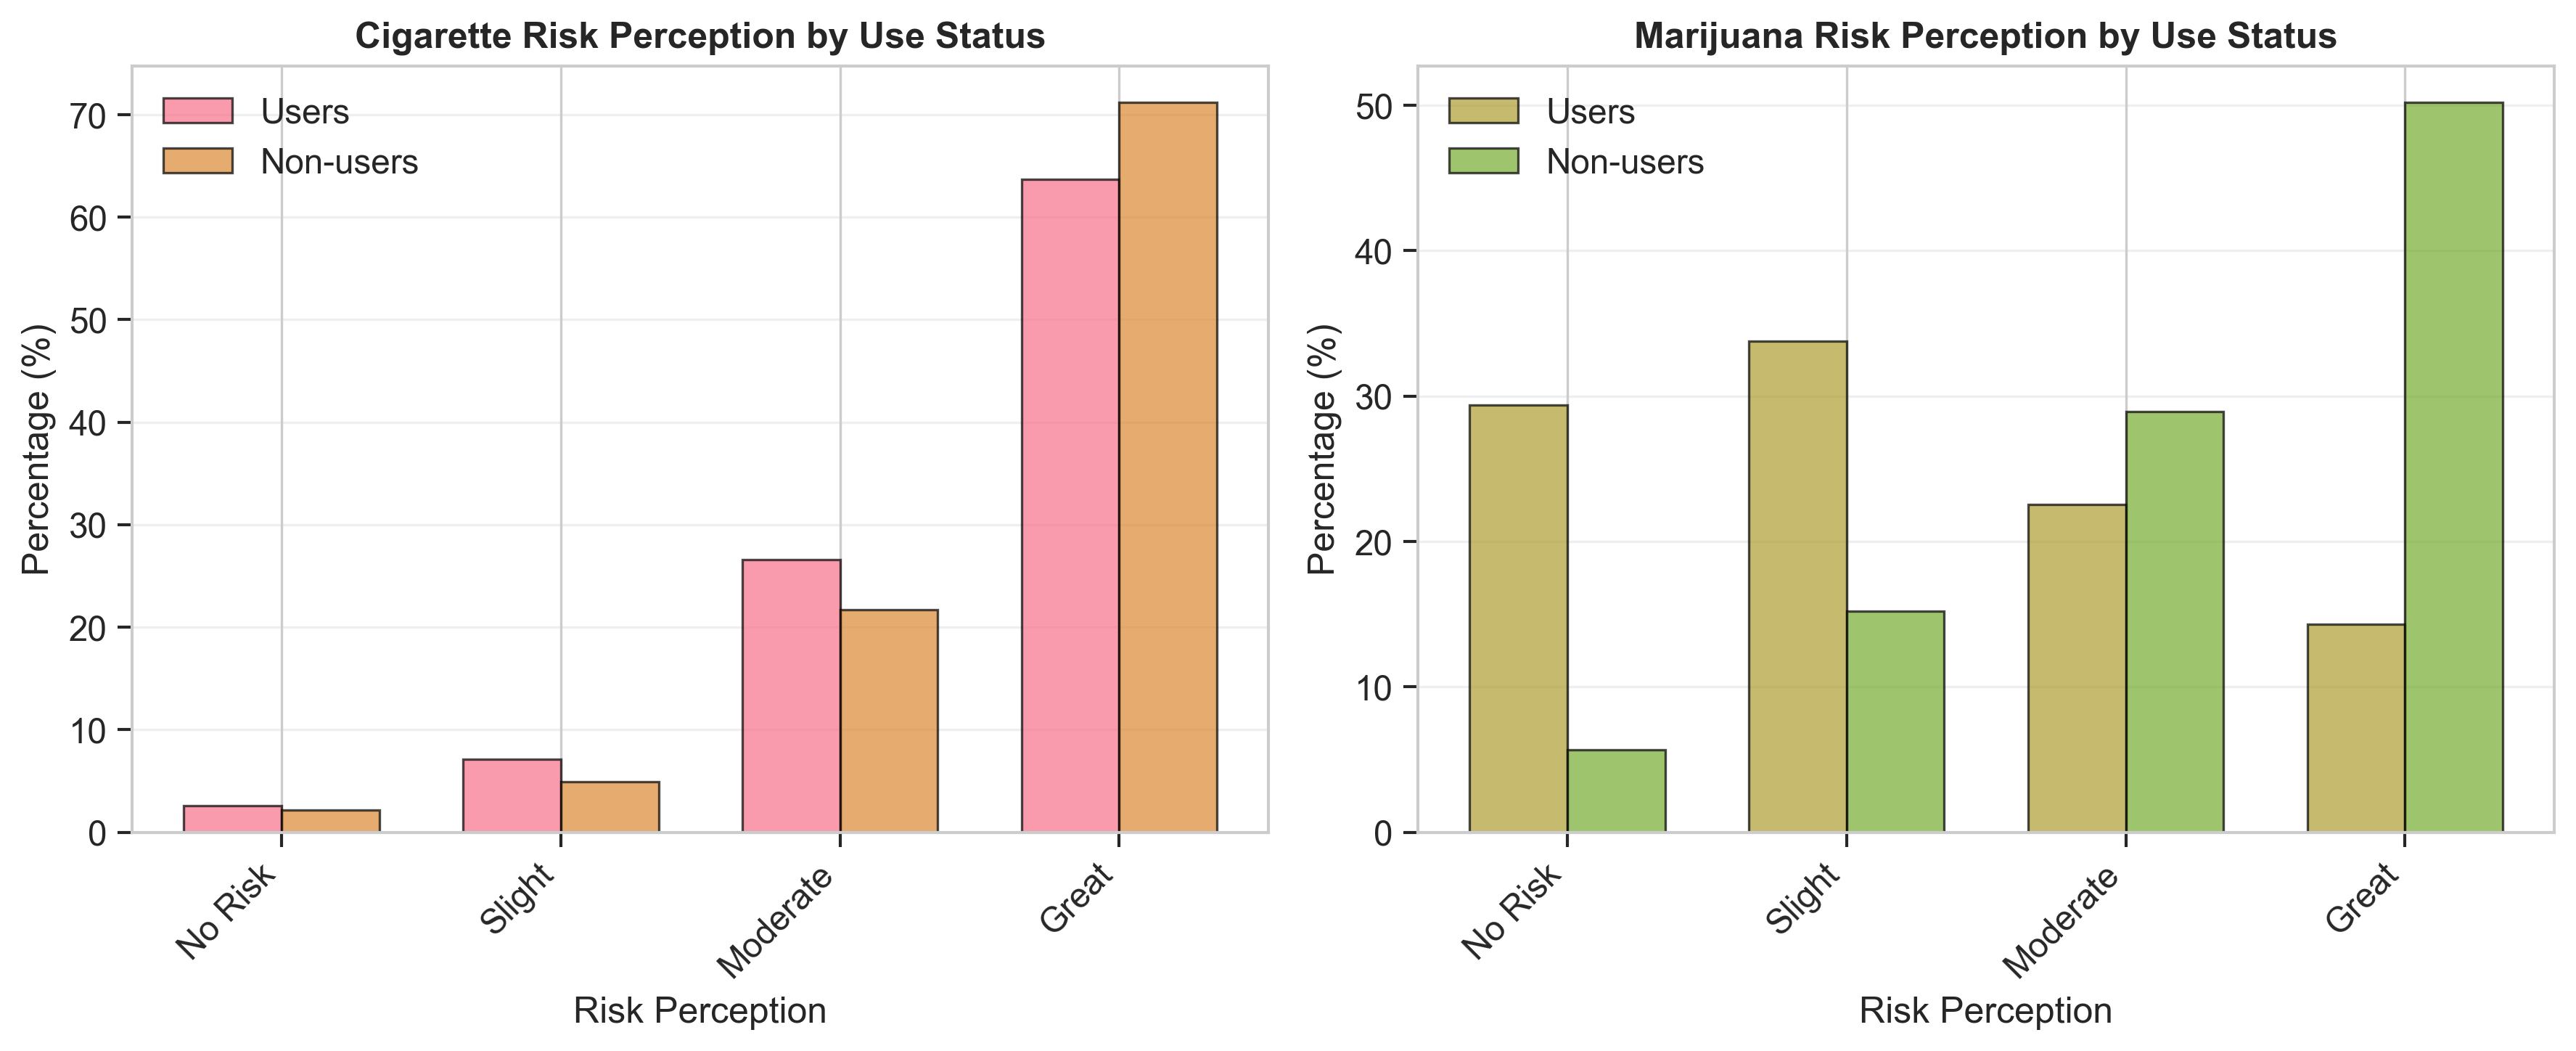
\includegraphics[width=\columnwidth]{figures/fig11_risk_perception_use.png}}
\caption{Risk perception distributions comparing users and non-users for cigarettes and marijuana.}
\label{fig:risk_use}
\end{figure}

For marijuana, the difference is more pronounced: users average 2.22 on the risk scale compared to 3.24 for non-users. Among marijuana users, 63.2\% perceive no or slight risk, compared to only 20.9\% of non-users. This suggests that lower risk perception is more strongly associated with marijuana use than cigarette use, possibly reflecting ongoing debates about marijuana's harms and benefits.

These findings suggest that risk communication strategies may need to be substance-specific. For cigarettes, where risk perception is already high, interventions might focus on other factors such as addiction or social norms. For marijuana, enhancing risk awareness may be more directly effective.

\subsubsection{RQ4: Dependence Patterns and Use Frequency}

Among cigarette smokers with complete dependence data (n=12,486), the mean dependence score was 5.18 (SD = 2.60) on a 2-10 scale. Pearson correlation analysis revealed a strong positive relationship between smoking frequency and dependence (r = 0.587, p $<$ 0.001), indicating that more frequent smoking is associated with greater dependence symptoms.

Figure \ref{fig:freq_dep} demonstrates this relationship through scatter plots and categorical comparisons. Daily smokers (25-30 days in past month) showed mean dependence scores of 6.41, compared to 3.07 for occasional smokers (1-10 days), a highly significant difference (t = 76.17, p $<$ 0.001).

\begin{figure}[htbp]
\centerline{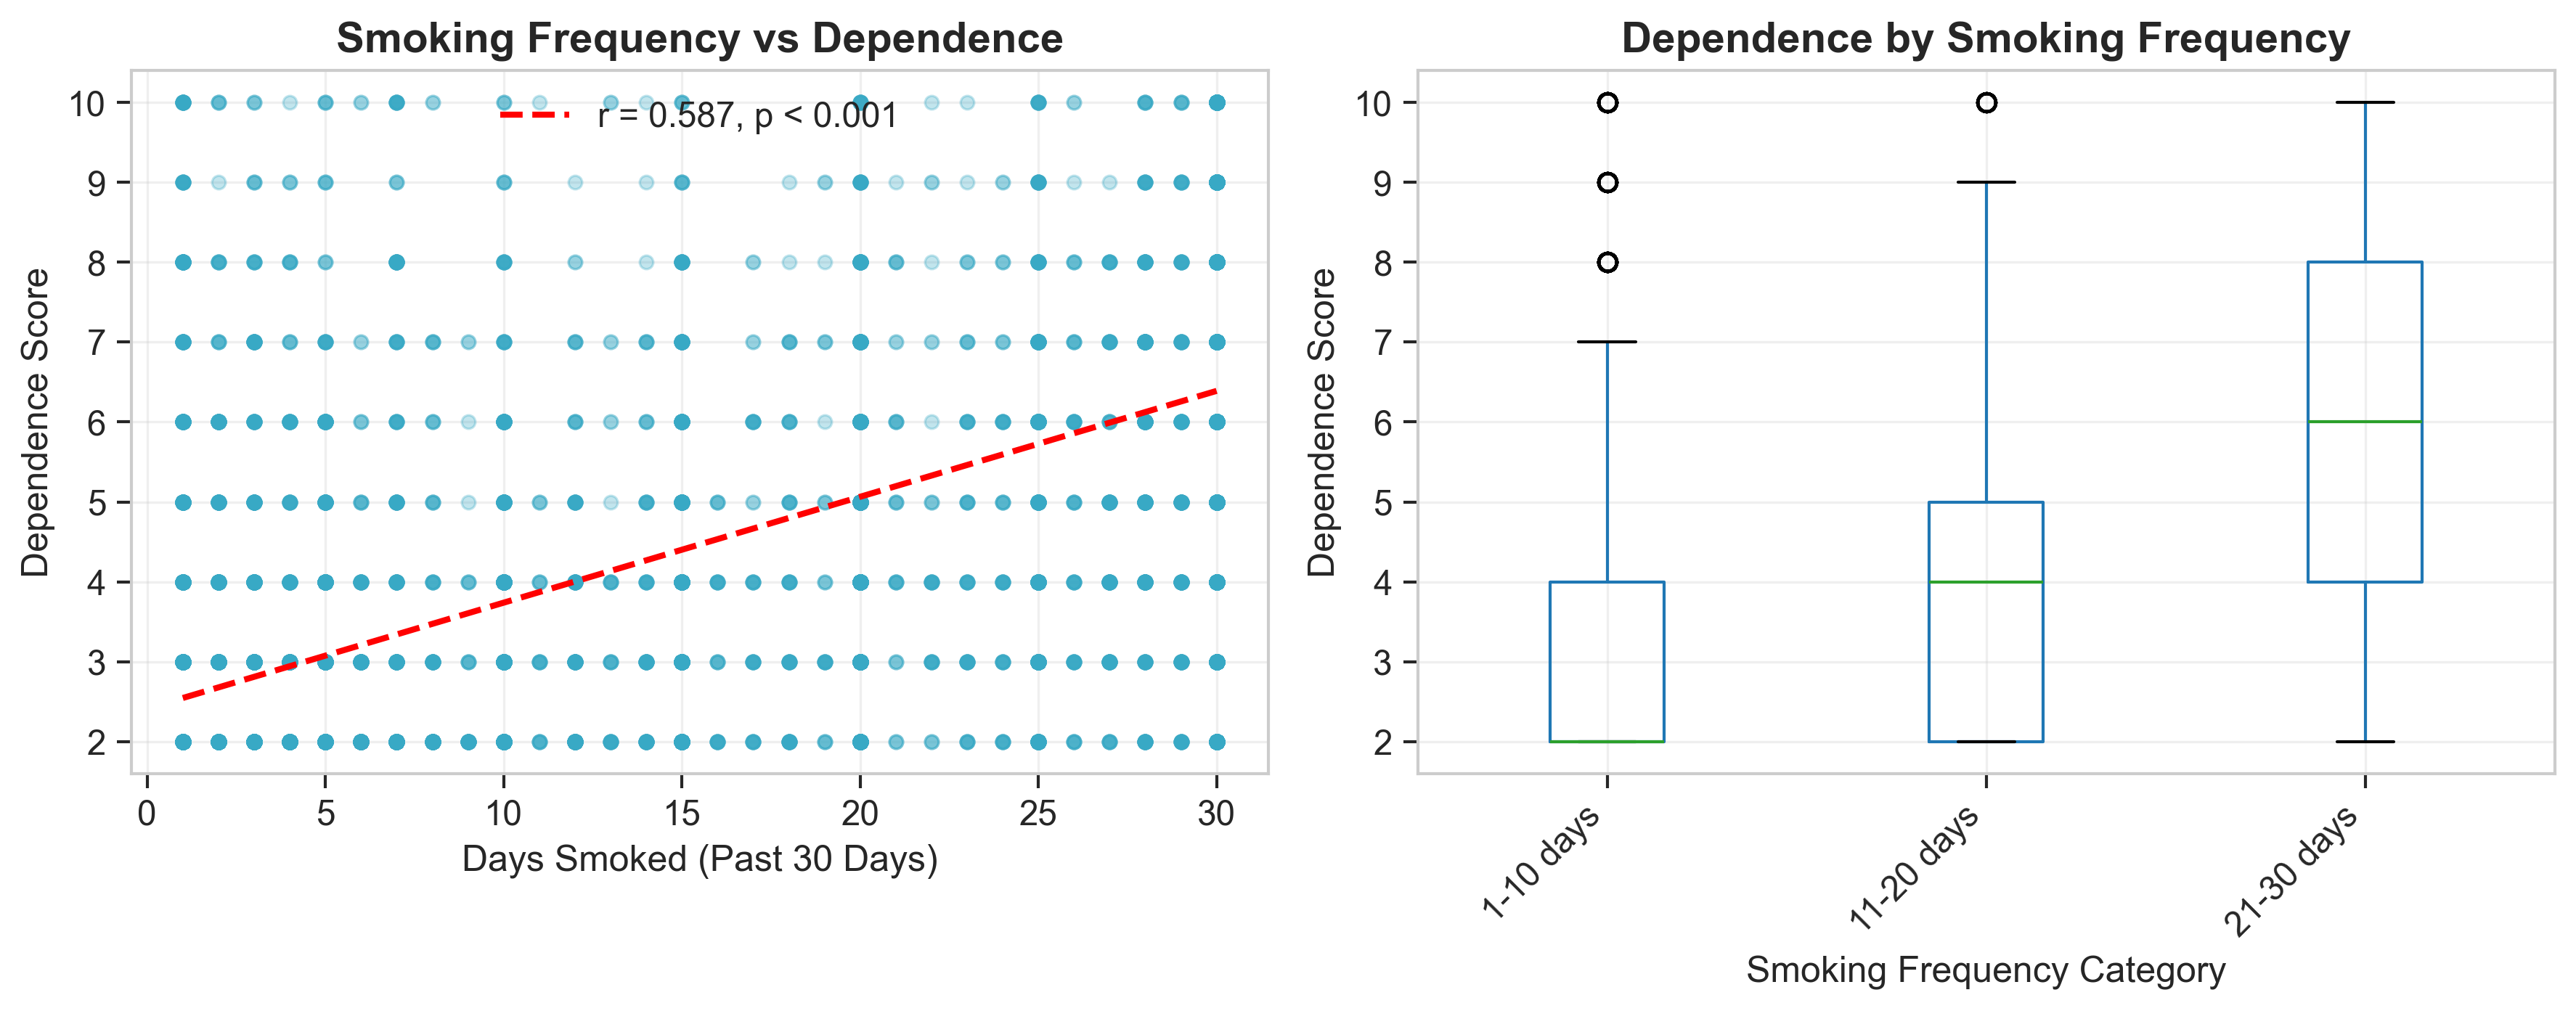
\includegraphics[width=\columnwidth]{figures/fig12_frequency_dependence.png}}
\caption{Relationship between smoking frequency and dependence scores, showing strong positive correlation (r = 0.587).}
\label{fig:freq_dep}
\end{figure}

The doubling of dependence scores from occasional to daily smoking underscores how quickly physiological dependence develops with regular use. This has important implications for cessation efforts, as daily smokers will likely require more intensive treatment support including potential pharmacotherapy.

\subsubsection{RQ5: Mental Health Correlates}

One-way ANOVA revealed significant differences in mental distress scores across substance use groups (F = 263.26, df = 3, p $<$ 0.001). Mean mental distress scores (scale: 3-15, higher = more distress) were: no substances (5.13), cigarettes only (5.14), marijuana only (5.48), and both substances (5.86).

Figure \ref{fig:mental} displays these patterns, showing that marijuana-only users and dual users experience significantly higher mental distress than cigarette-only or non-users. The additive effect observed for dual users (highest distress) suggests that polysubstance use may be particularly associated with mental health problems.

\begin{figure}[htbp]
\centerline{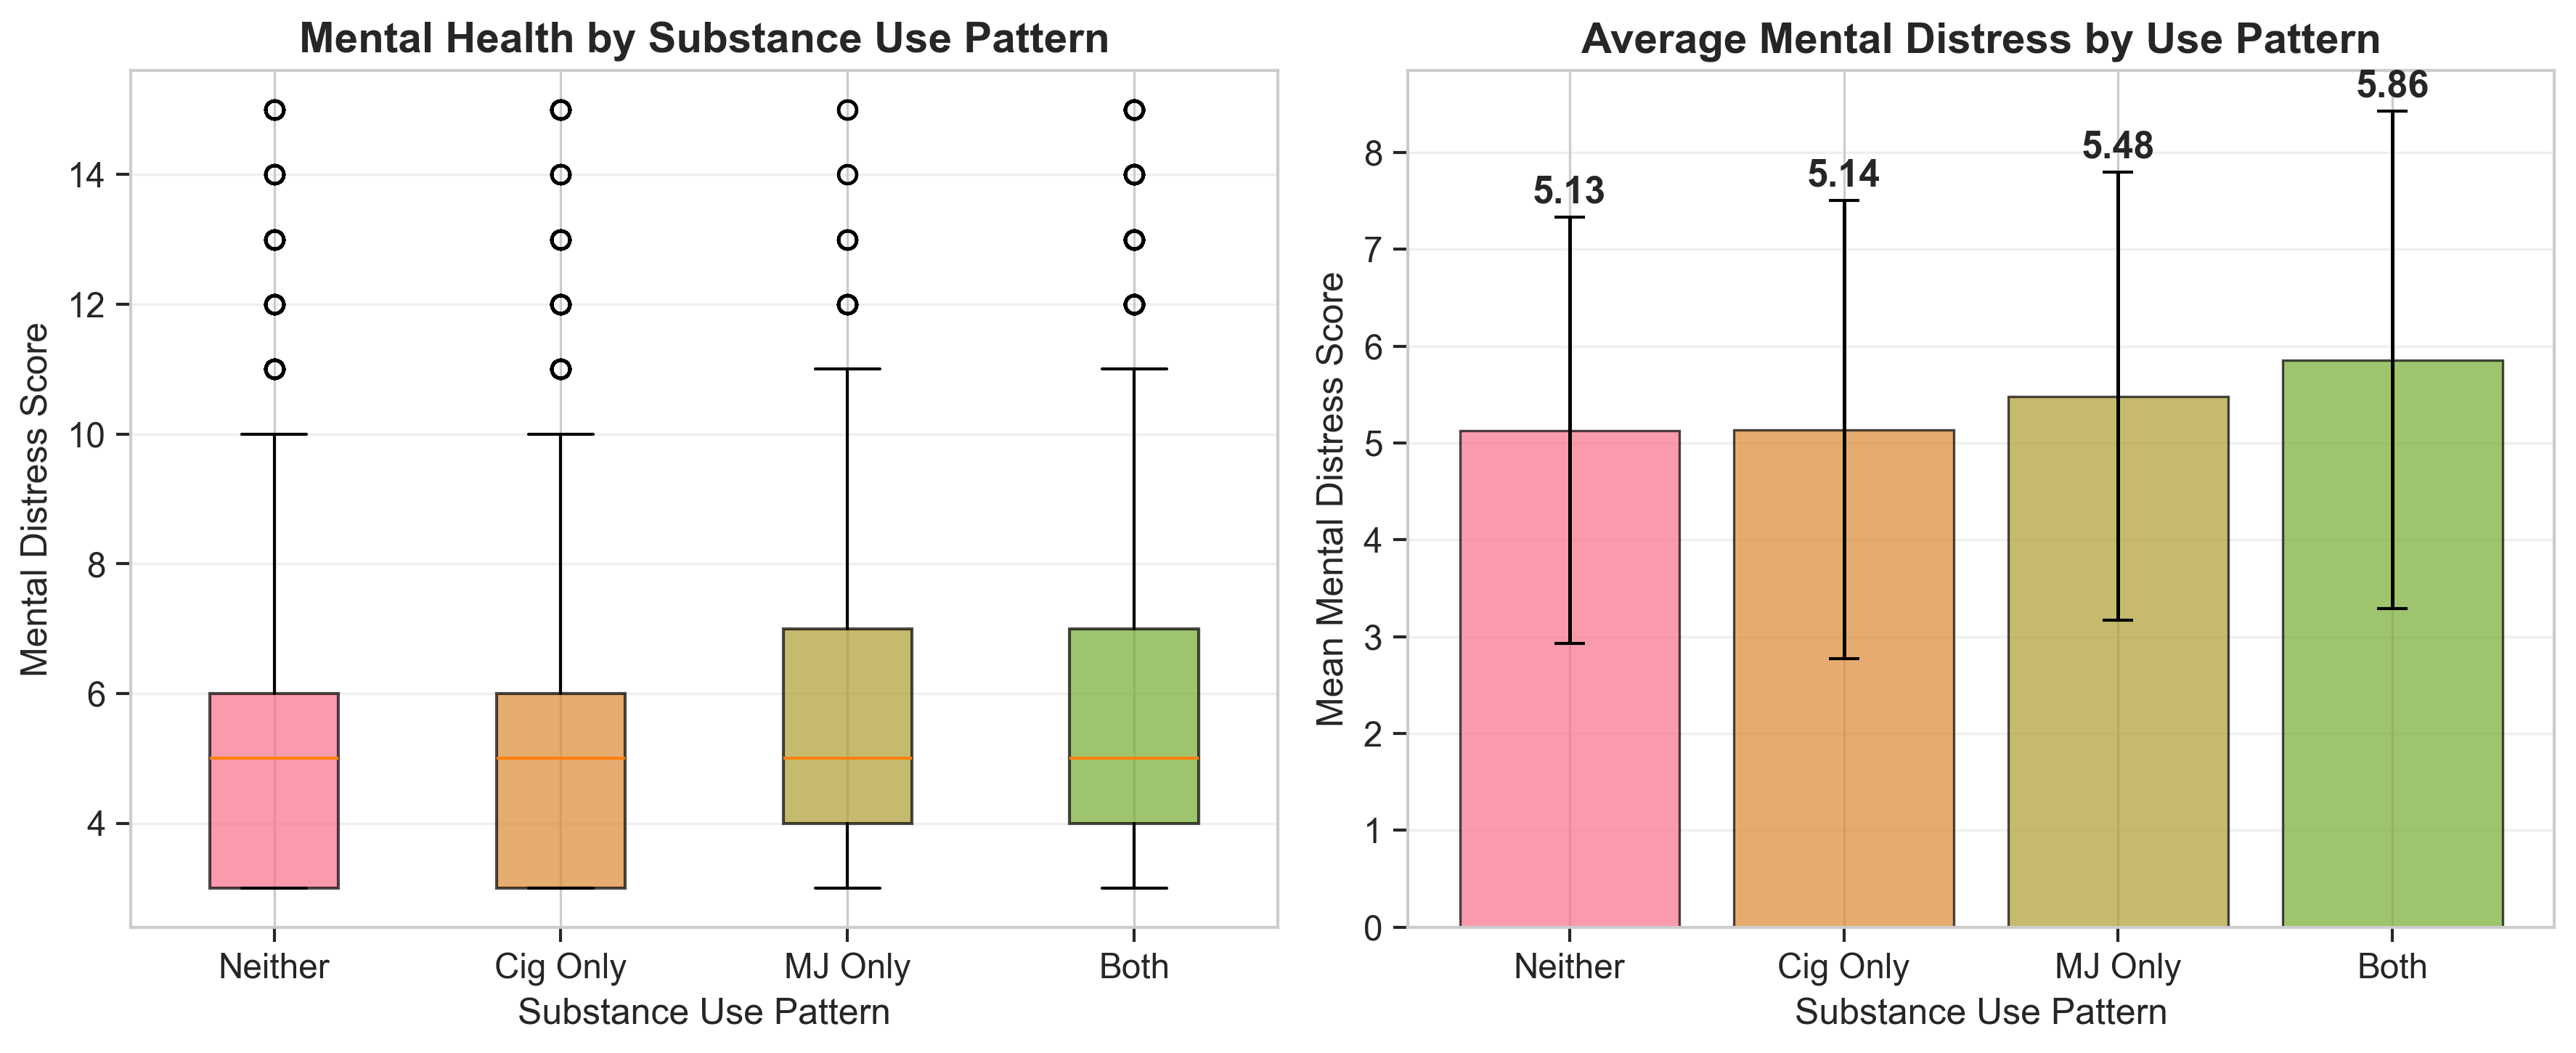
\includegraphics[width=\columnwidth]{figures/fig13_mental_health.png}}
\caption{Mental distress scores by substance use pattern, showing highest distress among dual users (ANOVA F = 263.26, p $<$ 0.001).}
\label{fig:mental}
\end{figure}

These findings are consistent with theories of self-medication, where individuals with mental health symptoms may use substances as coping mechanisms. However, the cross-sectional design precludes causal inference; it is equally plausible that substance use contributes to mental distress. The particularly high distress among dual users suggests that polysubstance use may either attract individuals with more severe mental health issues or compound mental health problems beyond single-substance use.

Clinical implications include the importance of integrated treatment approaches that address both substance use and mental health, and screening for mental health issues in substance abuse treatment settings.

\subsubsection{RQ6: Co-occurrence of Cigarette and Marijuana Use}

Chi-square analysis revealed a highly significant association between cigarette and marijuana use ($\chi^2$ = 17156.73, df = 1, p $<$ 0.001), with an odds ratio of 14.20. This indicates that the odds of having used marijuana are more than 14 times higher among cigarette users than among non-users, representing an extremely strong association. In terms of probabilities, 67.3\% of cigarette users have used marijuana compared to 12.7\% of non-users, a relative risk of about 5.3.

Figure \ref{fig:cooccur} illustrates the co-occurrence patterns. Of the total sample, 43.3\% used neither substance, 16.5\% used only cigarettes, 6.3\% used only marijuana, and 34.0\% used both. Among cigarette users, 67.3\% also used marijuana; among marijuana users, 84.4\% also used cigarettes.

\begin{figure}[htbp]
\centerline{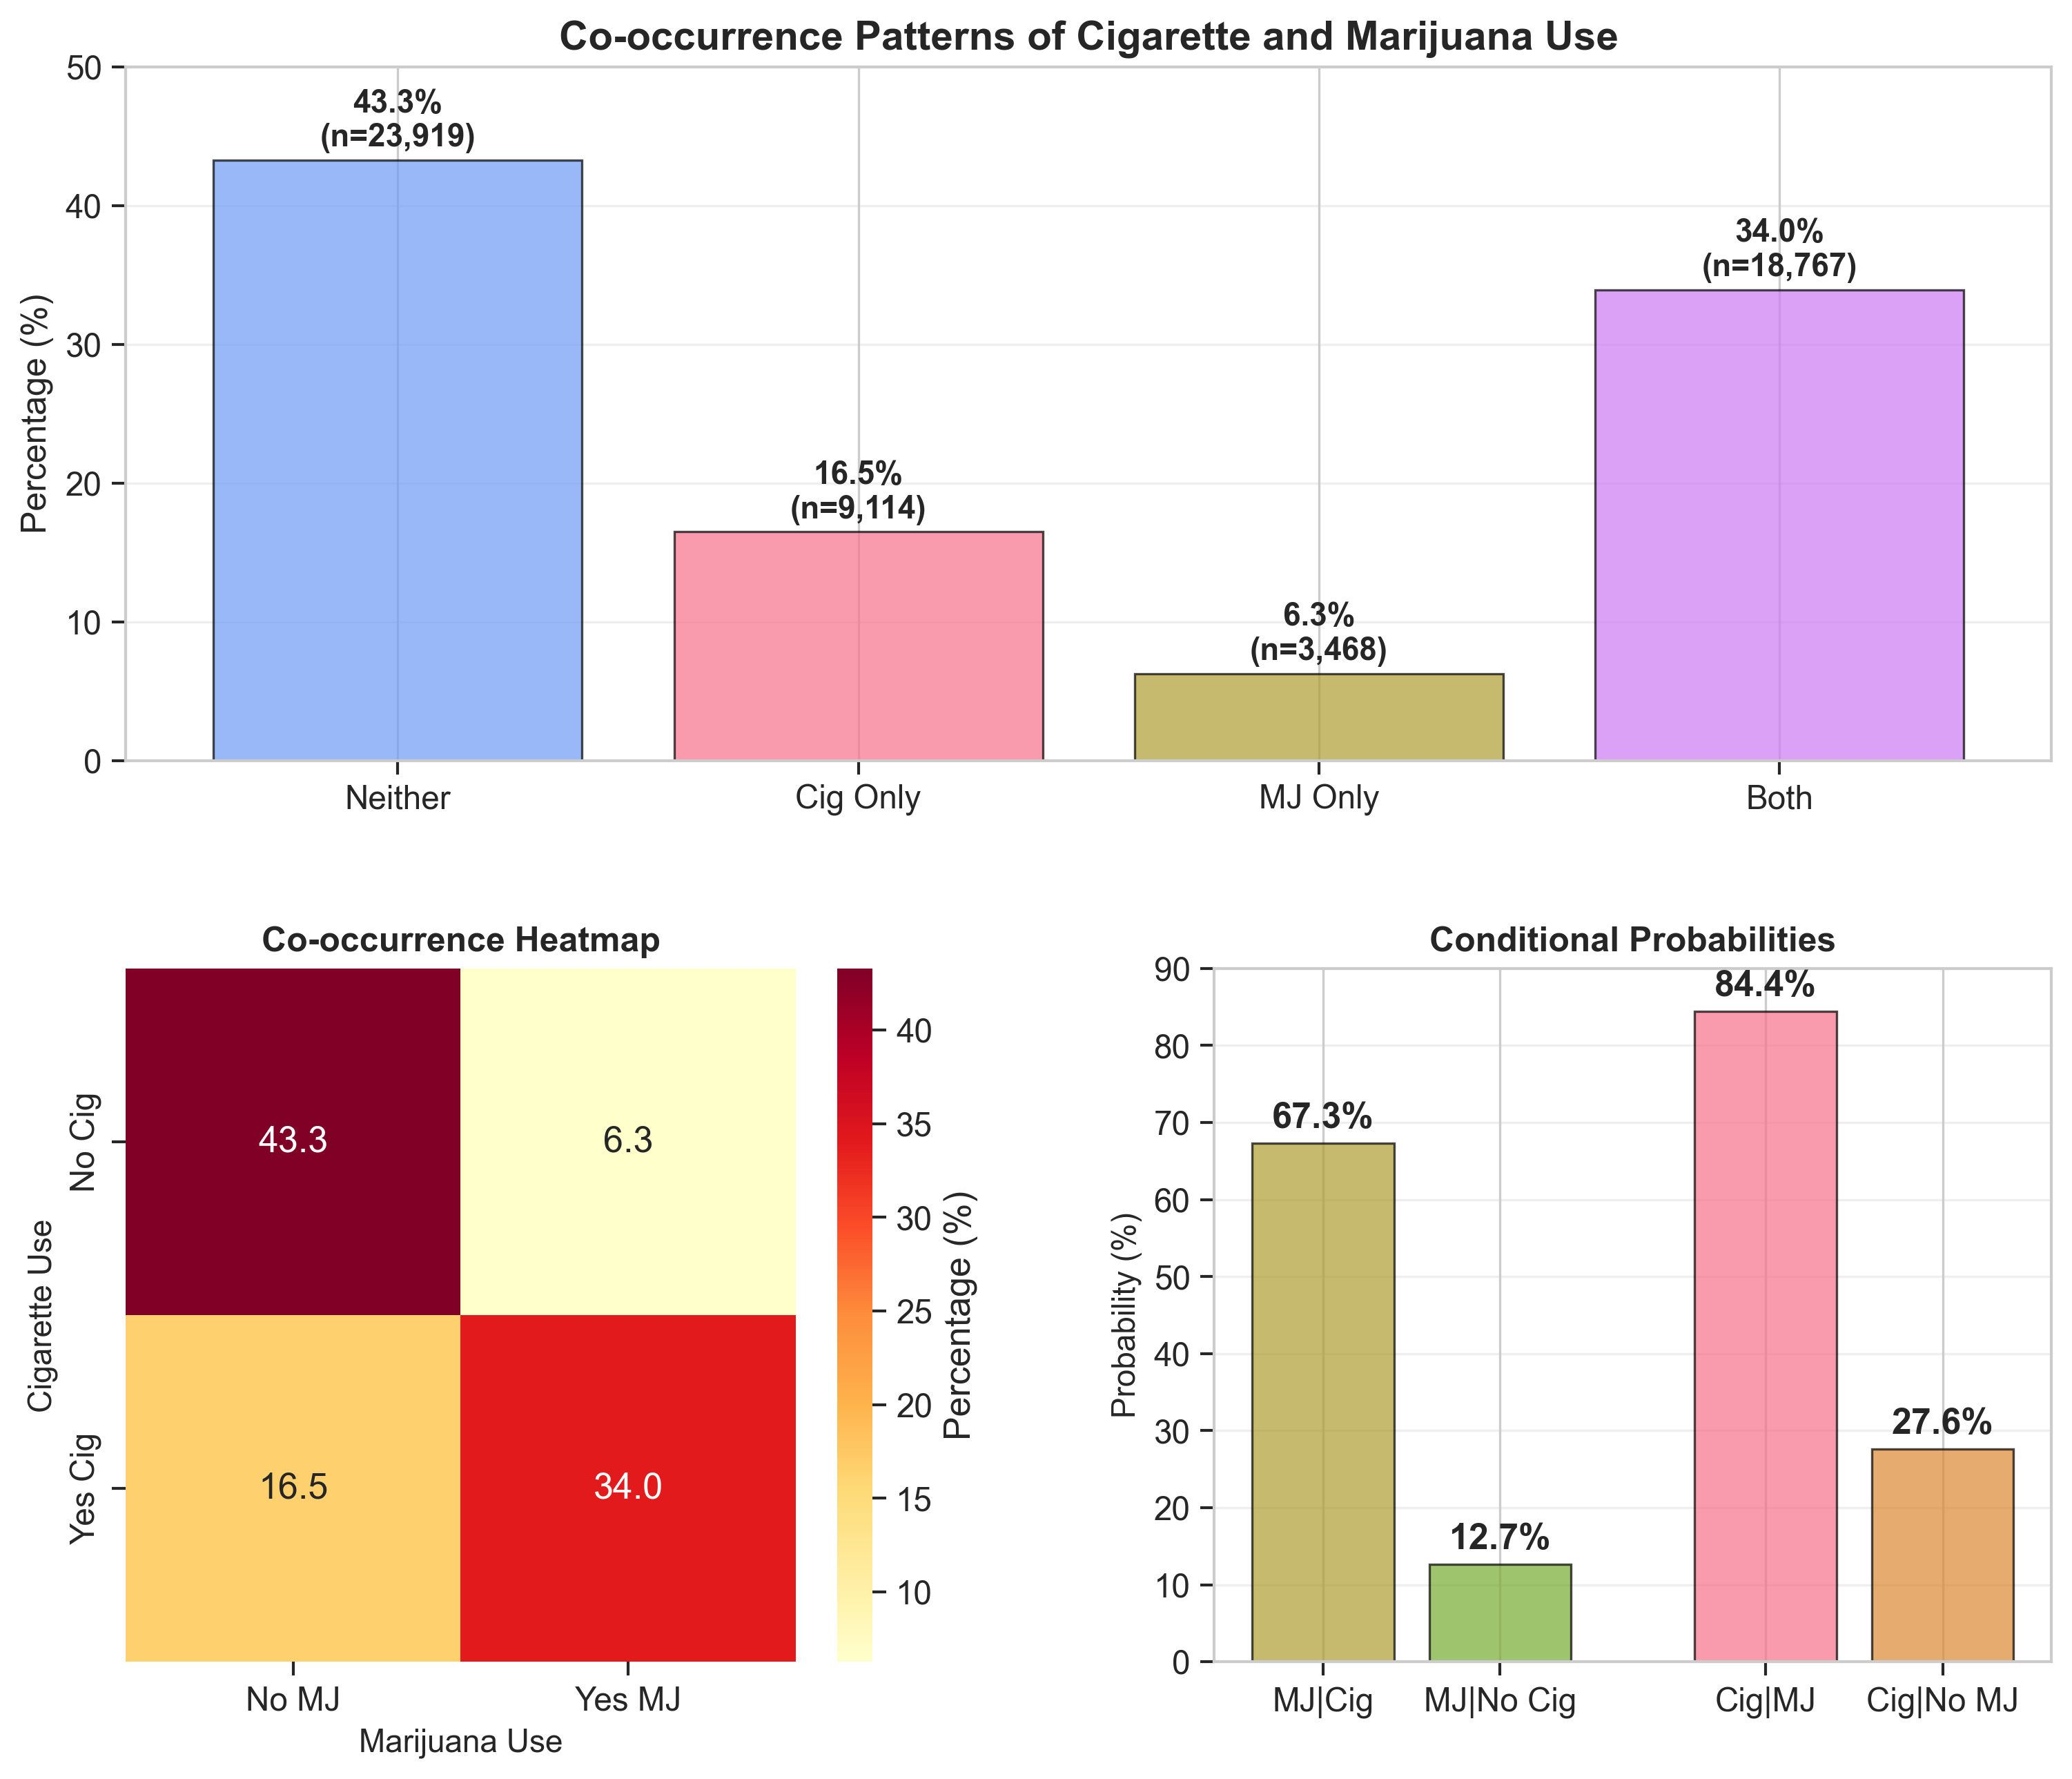
\includegraphics[width=\columnwidth]{figures/fig14_cooccurrence.png}}
\caption{Co-occurrence patterns showing strong association between cigarette and marijuana use (OR = 14.20, p $<$ 0.001).}
\label{fig:cooccur}
\end{figure}

The conditional probability analysis reveals asymmetric relationships: while most marijuana users also smoke cigarettes (84.4\%), a smaller majority of cigarette users also use marijuana (67.3\%). The relatively small proportion using only marijuana (6.3\%) suggests that marijuana-only use is uncommon, whereas cigarette-only use is more prevalent (16.5\%).

These findings have several important implications. First, the strong co-occurrence suggests common risk factors or causal pathways between the substances. The gateway hypothesis posits that cigarette use may facilitate marijuana use through social networks, behavioral patterns, or biological sensitization. Second, the findings highlight the need for integrated prevention and treatment approaches that address polysubstance use rather than focusing on single substances. Third, interventions targeting cigarette use may have spillover benefits for marijuana use prevention.

\section{Conclusion}

\subsection{Summary of Key Findings}

This comprehensive analysis of the NSDUH 2012 data has provided important insights into cigarette and marijuana use patterns in the United States. Our key findings include:

\textbf{Prevalence and Demographics}: Approximately half of Americans have tried cigarettes (50.4\%) and two-fifths have tried marijuana (40.2\%). Prevalence increases dramatically from adolescence to young adulthood, with the 18-25 age group showing particularly high rates. These patterns underscore the critical importance of prevention efforts targeting the adolescent-to-young-adult transition period.

\textbf{Initiation Patterns}: The mean age of first cigarette use (15.5 years) precedes marijuana initiation (16.5 years); among dual users, cigarettes are initiated approximately 1.3 years before marijuana (15.0 vs. 16.4 years). Males initiate both substances earlier than females, though differences are modest (4-6 months). The concentration of initiation during adolescence highlights this period as crucial for prevention.

\textbf{Risk Perception}: Inverse relationships exist between risk perception and use, particularly strong for marijuana (r = -0.461). While nearly all respondents recognize cigarette smoking as highly risky, marijuana risk perceptions are more varied and strongly differentiate users from non-users. These findings suggest that risk communication strategies should be tailored to specific substances.

\textbf{Dependence and Frequency}: Among cigarette smokers, frequency of use strongly predicts dependence symptoms (r = 0.587). Daily smokers show dependence scores more than twice those of occasional smokers (6.41 vs. 3.07), indicating rapid development of physiological dependence with regular use. This emphasizes the importance of early cessation interventions before daily smoking patterns become established.

\textbf{Mental Health}: Substance use is significantly associated with psychological distress, with marijuana-only users and particularly dual users showing elevated distress levels. These associations suggest important links between substance use and mental health that warrant integrated treatment approaches.

\textbf{Co-occurrence}: The extraordinarily strong association between cigarette and marijuana use (OR = 14.20) indicates substantial overlap between these behaviors. Over one-third (34.0\%) of the sample uses both substances, and among marijuana users, 84.4\% also smoke cigarettes. This pervasive co-occurrence highlights the need for integrated prevention and treatment strategies.

\subsection{Limitations}

Several limitations should be considered when interpreting these findings. First, the cross-sectional design precludes causal inference; associations observed may reflect selection effects, common antecedents, or bidirectional relationships rather than causal pathways. Longitudinal studies are needed to establish temporal ordering and test causal hypotheses.

Second, substance use data rely on self-report, which may be subject to social desirability bias and recall error. While the use of ACASI technology improves reporting of sensitive behaviors, some underreporting likely remains, particularly for stigmatized substances and among populations where use is less normative.

Third, all estimates are unweighted; because NSDUH oversamples younger respondents, sample percentages differ from population estimates. Mental health measures were available only for adults, so findings involving mental distress do not apply to adolescents.

Fourth, the public use file contains aggregated and top-coded variables for confidentiality protection, limiting the precision of some analyses. More detailed analyses would be possible with restricted-use data files.

Fifth, the survey excludes institutionalized populations (e.g., prison inmates, hospitalized individuals) and homeless persons not in shelters. These populations have higher substance use prevalence, so our findings may underestimate population-level use.

Sixth, our mental health measures assess general psychological distress rather than specific psychiatric diagnoses. More comprehensive mental health assessment would enable examination of relationships with specific disorders.

Finally, the data are from 2012; substance use patterns, particularly for marijuana, have evolved considerably in recent years with changing legalization policies. Updated analyses with recent data would be valuable for understanding current patterns.

\subsection{Future Work}

Several directions for future research emerge from this study. First, longitudinal analyses using multiple waves of NSDUH data could examine temporal sequences and developmental trajectories of substance use. Such analyses could test gateway hypotheses, identify predictors of escalation from experimental to regular use, and characterize patterns of desistance.

Second, predictive modeling using machine learning approaches could identify individuals at high risk for substance use initiation or progression to problematic use. Features predictive of risk could inform targeted prevention efforts and early identification systems.

Third, mediational analyses could examine mechanisms linking demographic factors, risk perceptions, and mental health to substance use behaviors. Understanding these pathways could identify intervention targets for prevention programs.

Fourth, comparative analyses across multiple survey years could document trends in use patterns, particularly for marijuana in the context of changing legal environments. Such trend analyses could evaluate the impacts of policy changes on population-level use.

Fifth, geographic analyses using state-level data could examine relationships between policy environments (e.g., marijuana laws, cigarette taxation), cultural factors, and use prevalence. Such analyses could inform evidence-based policy making.

Sixth, analyses incorporating genetic and biological data (in cohorts where available) could examine gene-environment interactions in substance use risk. Understanding biological vulnerabilities could enable precision prevention approaches.

Seventh, economic analyses examining relationships between substance use and employment, income, and healthcare utilization could quantify societal costs and inform resource allocation for prevention and treatment programs.

Finally, qualitative research complementing these quantitative findings could provide deeper understanding of subjective experiences, motivations for use, and barriers to cessation. Mixed-methods approaches combining population surveillance with in-depth interviews could provide comprehensive understanding of substance use behaviors.

\subsection{Implications for Practice and Policy}

These findings have several important implications for prevention, treatment, and policy:

\textbf{Prevention}: The concentration of initiation during adolescence and young adulthood indicates that prevention programs should be developmentally targeted, with school-based programs for adolescents and campus/community programs for young adults. The strong co-occurrence of cigarette and marijuana use suggests that integrated prevention programs addressing multiple substances may be more efficient than substance-specific programs.

\textbf{Risk Communication}: The findings regarding risk perception suggest that communication strategies should be substance-specific. For marijuana, where risk perception varies widely and strongly predicts use, enhancing risk awareness may be directly effective. For cigarettes, where risk perception is already high, alternative approaches focusing on addiction, social norms, or opportunity costs may be needed.

\textbf{Treatment}: The strong association between frequency and dependence underscores the importance of early intervention before daily use patterns become established. Treatment programs should incorporate mental health screening and services given the strong associations between substance use and psychological distress. The pervasive co-occurrence of cigarette and marijuana use indicates that treatment programs should address polysubstance use rather than single substances.

\textbf{Policy}: The age-related patterns in use suggest that policies restricting youth access to tobacco products are important. The findings regarding marijuana acquisition through social networks suggest that social supply reduction may be as important as commercial supply reduction. The mental health findings highlight the importance of integrating substance abuse and mental health services.

\subsection{Conclusion}

This comprehensive analysis of the NSDUH 2012 data has provided important insights into cigarette and marijuana use patterns, their demographic and psychological correlates, and their interrelationships. The findings underscore the public health significance of these substances, the importance of the adolescent and young adult periods for prevention, the strong co-occurrence between substances, and the associations with mental health. These results can inform evidence-based prevention, treatment, and policy approaches to reduce the substantial public health burden of substance use.

\section*{Acknowledgment}

The authors thank the Substance Abuse and Mental Health Services Administration (SAMHSA) for making the NSDUH data publicly available, the Research Triangle Institute for data collection and preparation, and the thousands of respondents who participated in the survey.

\begin{thebibliography}{00}
\bibitem{cdc2014} Centers for Disease Control and Prevention, ``Smoking and Tobacco Use; Fact Sheet; Health Effects of Cigarette Smoking,'' 2014.
\bibitem{samhsa2013} Substance Abuse and Mental Health Services Administration, ``Results from the 2012 National Survey on Drug Use and Health: Summary of National Findings,'' NSDUH Series H-46, HHS Publication No. (SMA) 13-4795, 2013.
\bibitem{johnston2013} L. D. Johnston et al., ``Monitoring the Future National Survey Results on Drug Use, 1975-2012: Volume I, Secondary School Students,'' Institute for Social Research, The University of Michigan, Ann Arbor, 2013.
\bibitem{kandel2002} D. B. Kandel and K. Chen, ``Extent of smoking and nicotine dependence in the United States: 1991-1993,'' \textit{Nicotine \& Tobacco Research}, vol. 2, no. 3, pp. 263-274, 2000.
\bibitem{ajzen1991} I. Ajzen, ``The theory of planned behavior,'' \textit{Organizational Behavior and Human Decision Processes}, vol. 50, no. 2, pp. 179-211, 1991.
\bibitem{khantzian1997} E. J. Khantzian, ``The self-medication hypothesis of substance use disorders: A reconsideration and recent applications,'' \textit{Harvard Review of Psychiatry}, vol. 4, no. 5, pp. 231-244, 1997.
\end{thebibliography}

\end{document}